\documentclass[12pt,foolscap]{report}

\usepackage[utf8]{inputenc}
\usepackage[left=1.5cm,right=1.5cm,top=1.5cm,bottom=1.5cm]{geometry}
\usepackage[cyr]{aeguill}
\usepackage[francais]{babel}
\usepackage{graphicx}
\usepackage{amsmath}
\usepackage{amssymb}
\usepackage{breqn}
\usepackage[squaren,Gray]{SIunits}
\usepackage{subcaption}
\usepackage{supertabular}
\usepackage{hyperref}
\usepackage{float}
\usepackage{breqn}
\usepackage{lscape}
\usepackage{enumitem}

\usepackage{titling} % Customizing the title section
%Configuration figure http://aty.sdsu.edu/bibliog/latex/floats.html
\renewcommand{\topfraction}{0.9}	% max fraction of floats at top
\renewcommand{\bottomfraction}{0.8}	% max fraction of floats at bottom
\setcounter{topnumber}{2}
\setcounter{bottomnumber}{2}
\setcounter{totalnumber}{4}     % 2 may work better
\setcounter{dbltopnumber}{2}    % for 2-column pages
\renewcommand{\dbltopfraction}{0.9}	% fit big float above 2-col. text
\renewcommand{\textfraction}{0.07}	% allow minimal text w. figs
\renewcommand{\floatpagefraction}{0.7}	% require fuller float pages
% N.B.: floatpagefraction MUST be less than topfraction !!
\renewcommand{\dblfloatpagefraction}{0.7}	% require fuller float pages

\graphicspath{{images/}}
\usepackage[section]{placeins}
\usepackage[colorinlistoftodos,prependcaption,textsize=tiny]{todonotes}
\usepackage{array}
\usepackage{makecell}
%% biber use
\usepackage[autostyle]{csquotes}
\usepackage[backend=biber,style=authoryear-icomp,sortlocale=de_DE,natbib=true,url=false, doi=true,eprint=false]{biblatex}
\addbibresource{bibproj.bib}



%----------------------------------------------------------------------------------------
%	TITLE SECTION
%------------------------------------------------------------------------------------
\title{GMC 721 - Rayonnement acoustique des structures}

\author{%
	\textsc{PROJET: CONCEPTION, FABRICATION ET VALIDATION }\\
	\textsc{D'UN ENCOFFREMENT ACOUSTIQUE} \\
	\textsc{Samuel Dupont  }\\ %\thanks{A thank you or further information} \\[1ex] 
	\textsc{Matricule : 16 070 591}\\ \\
	%\normalsize Université du Maine \\ % Your institution
	\normalsize \href{mailto:Samuel.S.dupont.etu@usherbrooke.ca}{Samuel.S.dupont.etu@usherbrooke.ca} \\ \\
	\textsc{Nambouri Yazid  }\\ %\thanks{A thank you or further information} \\[1ex] 
	\textsc{Matricule: 16 164 446}\\ \\
	%\normalsize Université du Maine \\ % Your institution
	\normalsize \href{mailto:Nambouri.Yazid@usherbrooke.ca}{Nambouri.Yazid@usherbrooke.ca}\\ \\
	\textsc{Professeur : Alain Berry}\\ \\
}

\date{\today \\ }


%%%%%%%%%%%%%%%%%%%%%%%%%%%%%%%%%%%%%%%%%%%%%%%%%%%%%%%%%%%%%%%%%%%%%%%%%%%%%%%%%%%%%%%%%%%%%
%%%%%%%%%%%%%%%%%%%%%%%%%%%%%%%%%%%%%%%%%%%%%%%%%%%%%%%%%%%%%%%%%%%%%%%%%%%%%%%%%%%%%%%%%%%%%
%%%%%%%%%%%%%%%%%%%%%%%%%%%%%%%%%%%%%%%%%%%%%%%%%%%%%%%%%%%%%%%%%%%%%%%%%%%%%%%%%%%%%%%%%%%%%
%%%%%%%%%%%%%%%%%%%%%%%%%%%%%%%%%%%%%%%%%%%%%%%%%%%%%%%%%%%%%%%%%%%%%%%%%%%%%%%%%%%%%%%%%%%%%
%%%%%%%%%%%%%%%%%%%%%%%%%%%%%%%%%%%%%%%%%%%%%%%%%%%%%%%%%%%%%%%%%%%%%%%%%%%%%%%%%%%%%%%%%%%%%
%%%%%%%%%%%%%%%%%%%%%%%%%%%%%%%%%%%%%%%%%%%%%%%%%%%%%%%%%%%%%%%%%%%%%%%%%%%%%%%%%%%%%%%%%%%%%



\begin{document}
	% Print the title
	\maketitle
	
	
	\chapter{Introduction et objectifs}
	\label{ch:objectif}
	
	\section{Objectifs du projet}
	L'objectif de ce projet est de concevoir et tester un encoffrement qui 
	permettra d'isoler le rayonnement d'une source de bruit blanc sur une 
	bande de fréquence de 100 Hz à 10 kHz. Notre but est d'obtenir une 
	insertion maximale (minimale de 15 dB) tout en ayant la plus faible masse possible d'encoffrement. \\
	
	La source sonore à isoler est un haut-parleur mid-range M-Audio Studiophile DX4 de dimension 21 cm en hauteur, 15 cm en largeur et 16 cm en profondeur pesant 5.4 kg. Le haut parleur sera installé en position verticale dans l'encoffrement comme indiqué dans la figure \ref{meas}. \\
	
	Afin de réaliser ce projet, nous serons limités à un budget maximal de 100\$ pour l'achat des matériaux devant servir à la fabrication de l'encoffrement. Nous serons aussi limité à seulement 1 m pour les dimensions extérieures dans les 3 directions hauteur, largeur et profondeur.
	
	\section{Critères d'évaluations}
	\label{sec:critereeval}
	Afin de pouvoir évaluer les performances du produit, on mesurera la pression sans encoffrement générée par la source $P_{i,sans} $, la pression avec encoffrement $P_{i,avec} $ et on utilisera les critères suivants:\\
	\begin{itemize}
		\item La perte par insertion en bande d'octave définie par : 
		\begin{align}
		IL_{\omega} &= 10\log_{10} (\frac{ \sum_{i}|P_{i,sans} \omega|^2 }{ \sum_{i}|P_{i,avec} \omega|^2 )}\text{.}
		\label{eq:ilo}
		\end{align}
		
		\item La perte par insertion globale définie par     :
		\begin{align}
		IL_{G} &= 10\log_{10} (\frac{\int \sum_{i}|P_{i,sans} \omega|^2 d\omega}{\int \sum_{i}|P_{i,avec} \omega|^2 d\omega})\text{.}
		\label{eq:ilg}
		\end{align}
		L'intégration sera faite sur la bande de fréquence de 100 Hz et 8 
		kHz.\\
		\item La perte par insertion globale pondérée par la masse défini par : 
		\begin{align}
		I{L_M} = I{L_G} - 10{\log _{10}}({M^2})
		\label{eq:ilm}
		\end{align}
		où M est la masse totale de l'encoffrement.\\
		
		\item La mesure des pressions acoustiques sera faite à 5 points 
		identifiés dans la figure \ref{meas}. 
	\end{itemize}
	\begin{figure}
		\centering
		\makebox[0pt]{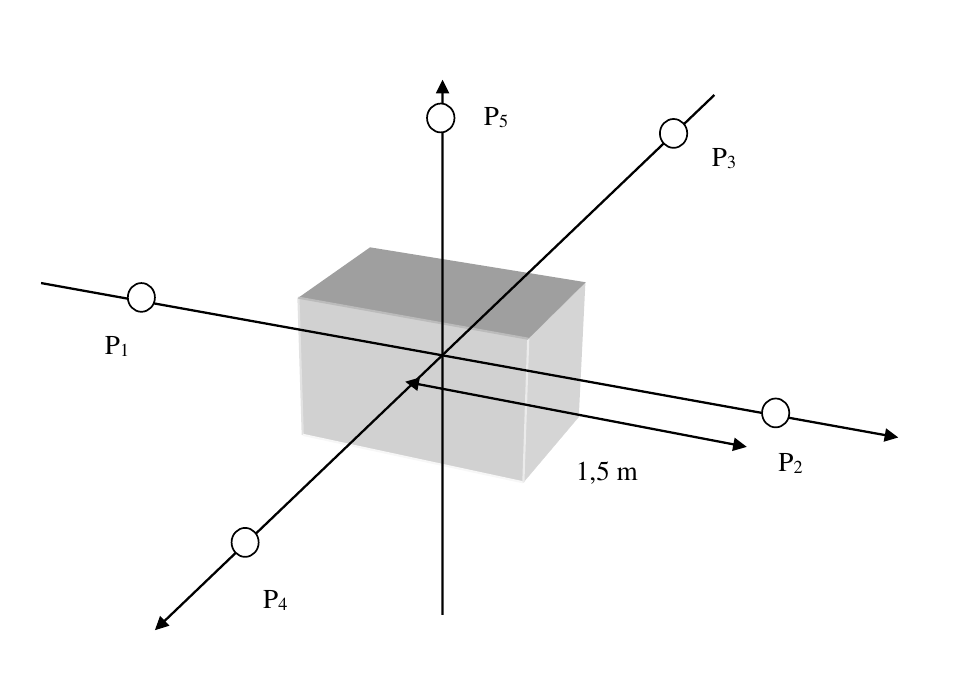
\includegraphics[width=450px]{images/obj/configmeas.png}}
		\caption{ Protocole de mesure de la performance acoustique d'un encoffrement.
		}
		\label{meas}
	\end{figure}
	
	\section{Généralités}
	Avant d'entamer les démarches suivies dans ce projet, on définit 
	d'abord certains pré-requis acoustiques dont on s'est servi pour la 
	réalisation de ce projet.\\ 
	\subsection*{La transparence} 
	La transparence acoustique est définie par: \\
	\begin{align}
	\tau (\omega ,\theta ) = \frac{{{I_t}(\omega ,\theta )}}{{{I_i}(\omega ,\theta )}}\text{,}
	\label{eq:transtau}
	\end{align}
	où \({I_t}\,{\rm{et}}\,{I_i}\) sont respectivement les intensités acoustiques de l'onde transmise et de l'onde incidente normales à la paroi, \(\theta \) l'angle d'incidence et \(\omega \) la pulsation de l'onde acoustique. \\
	
	Dans la réalité les sources sont rarement des ondes planes mono-incidente mais plutôt multi incidente. En prenant en compte ce fait on parle de champ diffus, la transparence en champ diffus est définie par: \\
	\begin{align}
	{\tau _d}(\omega ) = 2\int\limits_0^{\frac{\pi }{2}} {\tau (\omega ,\theta )\cos \theta \sin \theta d\theta } \text{.}
	\end{align}
	
	\subsection*{Affaiblissement} 
	L'indice d'affaiblissement est une mesure permettant de caractériser 
	l'affaiblissement du rayonnement acoustique d'une structure. Il est inversement proportionnel à la transparence acoustique et est 
	défini par la formule suivante, dans le cas mono incident par : \\
	\begin{align}
	R = 10{\log _{10}}\left( {\frac{1}{\tau }} \right)\text{.}
	\label{eq:affaibl}
	\end{align}
	\subsection*{Perte par insertion}
	La perte par  insertion en bandes 1/3 octave \(I{L_\omega}\) défini précédemment comme l'Éq. \ref{eq:ilg} et la perte par insertion $I{L_G}$  défini précédemment  Éq. \ref{eq:ilg} caractérisent la perte de son induite par l'encoffrement.\\
	En supposant un champ diffus, des pressions des ondes planes incidentes des ondes planes normalisés et en approximant un encoffrement comme une plaque infinie on peut réécrire la perte par insertion comme : \\
	\begin{align}
	IL(\omega) = 10{\log _{10}}\frac{1}{{{{\left| {{P_{i,avec}}(\omega )} \right|}^2}}}=10{\log _{10}}\left( {\frac{1}{\tau_d }} \right)\text{.}
	\end{align}
	Cette approximation est forte car on ne prend pas en compte ni l'effet de cavité, ni l'aspect fini des plaques, mais cependant nécessaire afin de pouvoir comparer nos résultats à ceux mesurés. Ces deux effets seront discutés dans le chapitre théorie. \\
	
	Les deux critères présentés  ne prennent en compte que l'affaiblissement acoustique dans la performance, or la masse de l'encoffrement joue beaucoup, en effet plus celle ci est élevé plus la réduction est naturellement importante, une pondération négative par la masse  définie par l'Éq \ref{eq:ilm} permet comparer l'optimisation d'une configuration  à une autre.
	
	
	
	
	\chapter{Théorie}
	L'entièreté des programmes est disponible sur Github à l'adresse suivante :\\
	\href{https://github.com/Nuopel/Encoffrement/tree/master/Programme}{https://github.com/Nuopel/Encoffrement/tree/master/Programme}. Pour utiliser les programmes il faut télécharger le dossier "fonction".
	\section{Hypothèses générales}
	
	On considérera la source comme ayant une directivité monopolaire, générant un champ diffus. Les parois de l'encoffrement sont modélisés sous forme de plaques infinies excitées par les ondes provenant de cette source. \\ \\
	On étudiera seulement des plaques infinies en considérant que chaque face de l'encoffrement pourrait se ramener à une seule plaque infinie et que toutes les parois subissent le même effet des ondes qui les traversent. \\ \\
	Pour passer de l'étude des plaques infinies aux plaques finies, on devra tenir compte du comportement modal des plaques, mais ceci étant plus complexe, on simplifiera le système en négligeant les effets de réflexion des ondes réfléchies par les bords des parois finies de l'encoffrement.\\ \\
	
	
	\section{Transmission acoustique par une cloison infinie}
	\begin{figure}[h!]	
		\centering
		\begin{minipage}[c]{.45\linewidth}
			\begin{center}
				\makebox[0pt]{\includegraphics[width=300px]{images/schemacloisons/simple_cloison.JPG}}
				\caption{ Schéma d'un système à cloison simple.}
				\label{simplecloison}
			\end{center}
		\end{minipage}
		\hfill
		\begin{minipage}[c]{.45\linewidth}
			\begin{center}
				\centering
				\makebox[0pt]{\includegraphics[width=300px]{images/th/compsimpleplaque.eps}}
				\caption{ Affaiblissement pour deux simples cloisons de $h_1$ = 6.4 mm et $h_{2}$ = 12.8 mm d'épaisseur, d'angle d'incidence $\theta  = 40^\circ $, $\rho  = 750 {\rm{Kg/}}{{\rm{m}}^3},{\rm{E = 3}}{\rm{GPa, }} \nu = $0.245 ,les fréquences de coïncidences sont notés par les traits verticaux rouges. \href{https://github.com/Nuopel/Encoffrement/blob/master/Programme/comparaison_cloison.m}{Lien prog.}}
				\label{simplecloin1}
			\end{center}
		\end{minipage}
	\end{figure}
	
	La figure \ref{simplecloison} représente la transmission acoustique dans une cloison infinie avec les propriétés suivantes données : une masse surfacique \(\mu \) , une rigidité de flexion D. L'onde \({p_i}\) de nombre d'onde k a une incidence \(\theta \). On note \({p_r}\) et \({p_t}\) respectivement les ondes réfléchies et transmises.
	La transparence pour cette cloison infinie est déterminée d'après le cours \cite{cours} par: \\
	\begin{align}
	\tau (\omega ,\theta ) = {\omega ^2}\frac{{{{({\rho _0}{c_0})}^2}}}{{{{\cos }^2}\theta }}\frac{4}{{{{\left| { - {\omega ^2}\mu  + Dk_0^4{{\sin }^4}\theta  + \frac{{2{\rho _0}\omega {c_0}}}{{j\cos \theta }}} \right|}^2}}}\text{.}
	\end{align} \\
	On note la pulsation de coïncidence par :\\
	\begin{align}
	{\omega _{coin}} = \frac{{c_0^2}}{{{{\sin }^2}\theta }}\sqrt {\frac{\mu }{D}} \text{,}
	\end{align} \\

	
	
	
	La pulsation de coïncidence définie où la transparence de la paroi est égale à 1 et l'indice d'affaiblissement est R = 0. C'est la fréquence à laquelle l'isolation de la paroi est mauvaise.\\ \\
	
	La fréquence de coïncidence est minimale en incidence rasante et est égale à la fréquence critique. Lorsque l'incidence diminue, elle augmente et est infinie en incidence normale \(\theta  = 0\). \\
	En incidence normale, l'indice d'affaiblissement est celui que prévoit la loi de masse.\\ \\
	La loi de masse indique que l'indice d'affaiblissement augmente de 6 dB en doublant la masse de la cloison. D'où en basse fréquence l'augmentation de la masse augmente l'indice d'affaiblissement mais diminue la fréquence de coïncidence de la cloison, ce qui peut être mauvais pour notre système car on ne veut pas avoir une fréquence de coïncidence dans une zone de très basse fréquence. De plus la performance de l'encoffrement sera jugée par sa masse, donc on veut avoir une faible masse possible pour avoir une bonne perte par insertion. \\ 
		
	De plus l'affaiblissement est faible pour le système à cloison simple et n'augmente pas assez rapidement pour bien isoler le bruit. \\
	Nous essayerons d'étudier le système à double cloison et observer la différence.\\
	
	
	
	
	\section{Transmission acoustique par une double cloison infinie}
	
	
	On considère le système constitué de 2 plaques (masse surfacique \(\mu \),\(\mu_2 \) , rigidité de flexion $D_1$, $D_2$) excité par une onde acoustique plane sous incidence oblique \(\theta \). Supposant que l'amplitude de cette onde de pression est unitaire et que le milieu acoustique est identique coté émetteur, coté récepteur et entre les 2 plaques (densité \({\rho _0}\) , célérité acoustique \({c_0}\) ) on peut établir les équations du système (équations pour la pression acoustique de chacun des 3 milieux, équations du mouvement des plaques, équations de continuité). \\ 
	Le schéma de ce système est représenté dans la figure \ref{cloisondouble}. \\
	\begin{figure}
		\begin{minipage}[c]{.45\linewidth}
			\begin{center}
				\makebox[0pt]{\includegraphics[width=300px]{images/schemacloisons/double_cloison.JPG}}
				\caption{Schéma d'une système à double cloison.}
				\label{cloisondouble}
			\end{center}
		\end{minipage}
		\hfill
		\begin{minipage}[c]{.45\linewidth}
			\begin{center}
				\makebox[0pt]{\includegraphics[width=300px]{images/th/compsimpledoubleplaque.eps}}
				\caption{Affaiblissement pour une double cloison en bleu de $h_1$ = 6.4 mm et $h_{2}$ = 12.8 mm d'épaisseur, d'angle d'incidence $\theta  = 60^\circ $, d'espacement 3cm, $\rho  = 750 {\rm{Kg/}}{{\rm{m}}^3},{\rm{E = 3}}{\rm{GPa, }} \nu = $0.245,les fréquences de coïncidences sont notés par les traits verticaux rouges, les fréquences de résonances inter-plaques par des traits verts et la fréquence de respiration par un trait noir.\href{https://github.com/Nuopel/Encoffrement/blob/master/Programme/doublecloison.m}{Lien prog.}}
				\label{w}
			\end{center}
		\end{minipage}
	\end{figure}	
	
	La démonstration qui permet d'obtenir le système d'équation  associé à une double cloison à été fait durant le devoir 6 du cours peut être retrouvé en annexe \ref{ch:demodev6}, le système obtenu est (en replaçant $\cos \theta$ par $\Theta$):
	\begin{align}	
	\begin{bmatrix}
	j k_0 \Theta    &0 & 0 &0&\rho_0\omega^2&0  \\
	0       & -j k_0 \Theta & j k_0 \Theta & 0 &\rho_0\omega^2 & 0  \\
	1       & -1 & -1 & 0 &-\mu \omega^2+Dk^4 & 0  \\
	0    &-j k_0 \Theta e^{-jk_0\Theta e}   & j k_0 \Theta e^{jk_0\Theta e}   &0&0&\rho_0\omega^2  \\
	0       & 0 & 0 &- j k_0 \Theta e^{-jk_0\Theta e} &0 & \rho_0\omega^2   \\
	0     & + e^{-jk_0\Theta e} & +e^{jk_0\Theta e} & - 	e^{-jk_0\Theta e} &0 & -\mu \omega^2+Dk^4  \\
	\end{bmatrix}
	\begin{Bmatrix}
	A_{ref} \\
	A_{tr2} \\
	A_{ref2}\\
	A_{tr3}\\
	C_{1} \\
	C_{2} 
	\end{Bmatrix}
	=\begin{Bmatrix}
	j k_0 \Theta \\
	0 \\
	-1\\
	0\\
	0 \\
	0
	\end{Bmatrix}
	\end{align}
	Il est possible de résoudre le système numériquement pour trouver les solutions et calculer l'indice d'affaiblissement Eq. \ref{eq:affaibl} à partir de la transparence acoustique : 
	\begin{equation}
	\tau = \frac{I_t(\omega,\theta)}{I_i(\omega,\theta)} = \frac{\frac{ \Re\{A_t^2\}}{2}\frac{cos\theta}{\rho_0 c_0}}{\frac{1}{2}\frac{cos\theta}{\rho_0 c_0}}=\Re \{A_t^2\}
	\end{equation}
	
	Pour éviter d'avoir un indice d'affaiblissement presque nul pour les fréquences de coïncidences de la cloison double identique, on étudiera un système double cloison d'épaisseurs différentes (air-cloison-air-cloison-air).
	
	La figure \ref{w} montre les résultats numériques de la cloison calculés précédemment comparés aux résultats analytiques des plaques simples.\\ On peut voir plusieurs différences apparaître entre les deux configurations. Des pics apparaissent, un en basse fréquence à 450 Hz (trait noir) et des harmoniques de 1980 Hz (traits verts). Le pic en basse fréquence peut être interprété comme le moment où les deux plaques vibrent en opposition de phase, créant une fréquence dite de respiration.\\
	Les fréquences harmoniques sont probablement dues à la présence d'ondes stationnaires entre les deux plaques, les murs imposent une condition limite de résonance demi-onde qui se répète à chaque harmonique.\\ 
	Enfin un mot général sur l'affaiblissement, on constate que les performances en très basse fréquences tendent à zéro, mais sont amélioré de quasiment 6 dB par rapport à la plaque simple tout   en suivant la loi de 6 dB par octave jusqu'à la fréquence de respiration où l'absorption devient minimale. La pente de la cloison double change pour devenir une pente de 12dB par octave. Le comportement aux fréquences de coïncidences met en avant que chacune des plaques simples limite la chute d'affaiblissement, chaque creux s'arrête à l'affaiblissement de l'autre plaque simple. Il en va de même pour les fréquences de résonances demi ondes qui s'arrêtent à l'affaiblissement d'une des deux plaques simples.\\
	Les problèmes majeurs de la plaque double sont la fréquence de respiration, et les fréquences de résonances demi-ondes. En rajoutant de l'amortissement dans la plaque (plus réaliste) et des matériaux absorbant, on devrait en réduire l'influence, rajouter une plaque pourrait aussi limiter ces facteurs.
	
	
	\section{ Transmission acoustique par une triple cloison infinie (3 plaques)}
	Afin de choisir la configuration finale pour la confection de l'encoffrement, on essaie aussi d'étudier la transmission des ondes acoustiques par triple cloison.\\
	Le système est illustré dans la figure \ref{tricloison}. \\
	
	\begin{figure}[h]
		\begin{minipage}[c]{.45\linewidth}
			\begin{center}
				\makebox[0pt]{\includegraphics[width=450px]{images/schemacloisons/triple_cloison.JPG}}
				\caption{ Schéma d'un système à triple cloison.}
				\label{tricloison}
			\end{center}
		\end{minipage}
		\hfill
		\begin{minipage}[c]{.45\linewidth}
			\begin{center}
				\makebox[0pt]{\includegraphics[width=300px]{images/th/comptripledoubleplaque.eps}}
				\caption{Affaiblissement pour une triple cloison en bleu de $h_1$ = 6.4 mm, $h_{2}$ = 12.8 mm, $h_{3}$ = 19 mm d'épaisseurs, d'angle d'incidence $\theta  = 40^\circ $,d'espacement 3cm et 4cm de chaque coté, $\rho  = 750 {\rm{Kg/}}{{\rm{m}}^3},{\rm{E = 3}}{\rm{GPa, }} \nu = $0.245,les fréquences de coïncidences sont notés par les traits verticaux rouges. \href{https://github.com/Nuopel/Encoffrement/blob/master/Programme/triplecloison.m}{Lien prog.}}
				\label{w2}
			\end{center}
		\end{minipage}
	\end{figure}
	
	De la même manière que pour la cloison double on peut partir des équations de continuités pour trouver le système d'équations régissant les amplitudes des différentes ondes. La démonstration est mise en annexe \ref{ch:demotriple}.
	Sous forme de système on obtient en remplaçant , $e^{-jk\cos \theta e}$ par $\alpha_{ep}$, $e^{+jk\cos \theta e}$ par $\alpha_{em}$,  $e^{-jk\cos \theta L}$ par $\alpha_{Lm}$, $e^{+jk\cos \theta e}$ par $\alpha_{Lp}$ et $jk_0\cos\theta$ par $x$:
	\begin{align}	
	\begin{bmatrix}
	x   &0 & 0 &\rho_0\omega^2&0&0&0&0&0  \\
	0       & -x & x  &\rho_0\omega^2 & 0&0&0&0&0   \\
	1       & -1 & -1  &D_1k^4-\mu_1 \omega^2 &  0&0&0&0&0  \\
	0    &-\alpha_{em}   & \alpha_{ep}&0   &0&0&\rho_0\omega^2&0&0 \\
	0       & 0 & 0 &0&-x\alpha_{em}   & x\alpha_{ep} & \rho_0\omega^2&0&0  \\
	0     &\alpha_{em}   & \alpha_{ep} &0 &-\alpha_{em}   & -\alpha_{ep}& D_2k^4-\mu_2 \omega^2&0&0  \\
	0&0&0&0&-x\alpha_{Lm}   & x\alpha_{Lp}&0&0&  \rho_0\omega^2\\
	0&0&0&0&0&0&0&-x\alpha_{Lm} &  \rho_0\omega^2\\
	0&0&0&0&\alpha_{Lm}&\alpha_{Lp}&0&-\alpha_{Lm} &  D_3k^4 -\mu_3 \omega^2\\
	\end{bmatrix}
	\begin{Bmatrix}
	A_{ref} \\
	A_{tr2} \\
	A_{ref2}\\
	C_{1} \\
	A_{tr3}\\
	A_{ref3}\\
	C_{2} \\
	A_{tr4}\\
	C_{3} 
	\end{Bmatrix}
	=\begin{Bmatrix}
	x\\
	0 \\
	-1\\
	0\\
	0 \\
	0\\
	0\\
	0\\
	0
	\end{Bmatrix}
	\end{align}
	
	
	Il est possible de résoudre le système numériquement pour trouver les solutions et calculer l'indice d'affaiblissement de la même manière que pour la double cloison. La figure \ref{w2} représente l'indice d'affaiblissement pour une configuration triple calculé numériquement. La réponse devient de plus en plus complexe, mais on retrouve les fréquences de coïncidences des trois plaques, les fréquences de résonances demi-ondes sur la triple plaque sont une combinaison des résonances des deux plaques. Il apparait en basse fréquence deux fréquences de respirations.\\
	Les performances globales en sont grandement amélioré surtout dans les fréquences médium. Le gros problème reste l'apparition des deux fréquences de respiration qui rendent le système moins performant en basse fréquence que les cloisons doubles.\\ Il faut noter que le fait de choisir des espacements et épaisseurs irréguliers limite les chutes d'affaiblissement.
	
	\section{Matrice de transfert (MT)}
	La méthode précédente est plutôt longue pour écrire les équations en prenant en compte l'amortissement ou plusieurs plaques, la méthode suivante permet un écriture plus simple et rapide.\\ 
	La méthode des matrices de transferts permet de décrire la propagation d'une onde dans un milieu, qu'il soit fluide, solide ou poreux. Elle permet de relier les pressions et vitesses de part et d'autre des couches et ainsi d'en obtenir  la réponse.\\
	On limite la représentation de la couche à une matrice $2\text{x}2$, en considérant une onde plane traversant le milieu d'épaisseur finie $h$, avec un angle d'incidence $\theta$.\\
	La symétrie du problème permet de déduire les autres directions. On peut ainsi définir le champ acoustique en un point $M$ en utilisant la pression acoustique $P$ et la vitesse particulaire $v_x$ à un point $M'$. Le vecteur d'état formé par ces deux composants est noté $V$.  La matrice de transfert $[T_{gd}]$
	permet d'écrire la relation  entre les vecteurs d'état de part et d'autre du milieu fini considéré :
	\begin{align}
	\begin{split}
	V(M)&=[T_{gd}]V(M')\\
	\begin{bmatrix}
	P(M)\\v_x(M)
	\end{bmatrix}&=
	\begin{bmatrix}
	T_{11} &T_{12}\\
	T_{21} &T_{22}
	\end{bmatrix}
	\begin{bmatrix}
	P(M')\\v_x(M')
	\end{bmatrix}\text{.}
	\end{split}
	\end{align}  
	Tout l'intérêt des matrices de transferts réside dans le cas multi-couches, où le  vecteur $V(M)$ s'écrit en fonction de la multiplication des matrices associées au différentes couches :
	\begin{align}
	\begin{split}
	V(M)&=[T_{1}][T_{2}][T_{3}][T_{\dots}]V(M')\\
	&=[T]V(M')\\&=
	\begin{bmatrix}
	T_{11} &T_{12}\\
	T_{21} &T_{22}
	\end{bmatrix}
	\begin{bmatrix}
	P(M')\\v_x(M')
	\end{bmatrix}\text{,}
	\end{split}
	\end{align}  
	où $[T]$ est une matrice globale $[2\text{x}2]$ reliant la couche d'entrée à la couche de sortie.
	\subsection{Cas d'une couche fluide équivalente}
	Comme présenté dans le livre \cite{allard_propagation_2009}, chapitre 11, le cas d'une couche fluide ou poreuse dotée d'un comportement fluide-équivalent, le champ acoustique est décrit par la pression acoustique $P(M )$ et la composante $v_x (M )$ de la vitesse acoustique selon l'axe $x$ :
	\begin{equation}
	V(M)=\begin{bmatrix}
	P(M)\\
	v_x(M)\\
	\end{bmatrix}
	\end{equation}
	La couche poreuse est pour sa part caractérisée par sa densité dynamique $\rho$, son épaisseur $h$ et la composante
	selon l'axe $x$ du nombre d'onde dans le fluide $k_x= (k_f^2-k_f^2\sin^2\theta)^{1/2}$. On a :
	
	\begin{equation}
	[T_{fluide}] = \begin{bmatrix}
	\cos(k_xe) & j\frac{Z_f }{\cos\theta}\sin(k_xe)\\
	j\frac{\cos\theta}{Z_f }\sin(k_xe) &  \cos(k_xe)
	\end{bmatrix} 
	\end{equation}
	
	\subsection{Cas d'une couche  élastique fine}
	En considérant un plaque fine avec une onde plane incidente $\theta$. L'impédance de la plaque $Z_p$ est définie par le ratio $(p_1- p_2)/v_p$. En considérant la continuité des vitesses normales de part et d'autre de la plaque on peut écrire la matrice de transfert $[T_{plaque}]$, d'après le mémoire Master de Dhia KERKENI \cite{thesis1}:
	\begin{equation}
	\begin{bmatrix}
	p_1 \\v_1
	\end{bmatrix}=
	\begin{bmatrix}
	1 &Z_p\\
	0 &1\\
	\end{bmatrix}
	\begin{bmatrix}
	p_2 \\v_2
	\end{bmatrix} \text{,}
	\end{equation}
	où l'expression de $Z_p$ donné par \cite{vigran2008room} est :
	\begin{equation}
	Z_p =  \frac{D}{j\omega}\left[k^4\sin^4\theta-k_p^2 \omega^{3/2}\right]\text{,}
	\end{equation}
	avec  $k$ nombre d'onde dans le fluide, $\theta$ l'angle d'arrivée dans le fluide,$D$ la rigidité de flexion et $k_p$ le nombre d'onde dans la plaque donnés par:
	\begin{equation}
	D = \frac{E h^3}{12(1-\nu^2)}\text{,}
	\end{equation}
	\begin{equation}
	k_p = \sqrt[4]{\omega}\sqrt{\mu/D}\text{.}
	\end{equation}
	
	\subsection{Lien avec l'indice d'affaiblissement}
	L'indice d'affaiblissement a déjà été défini précédemment par le ratio d'énergie transmise et incidente. Dans le cours GMC 721 \cite{cours}, il est montré que le l'énergie acoustique peut être écrite comme $ I = \frac{1}{2}\Re\left\lbrace p^*v \right\rbrace$, qui peut être réécrit avec $Z_c=p/v$ par 
	\begin{equation}
	I = \frac{1}{2}\Re\left\lbrace\frac{ p^*p }{Z_c}\right\rbrace = \frac{\left|p\right|^2}{2}\Re\left\lbrace\frac{ 1 }{Z_c}\right\rbrace\text{.}
	\label{eq:energie}
	\end{equation}
	En insérant l'Éq. \ref{eq:energie} dans la définition de la transparence acoustique \ref{eq:transtau}on obtient : 
	\begin{equation}
	\tau =  \frac{\left|p_t\right|^2}{\left|p_i\right|^2}\frac{ \Re\left\lbrace Z_{c1} \right\rbrace}{\Re\left\lbrace Z_{c2}\right\rbrace}\text{,}
	\label{eq:Tautrans2}
	\end{equation}
	où $Z_{c1}$ représente l'impédance caractéristique du coté de l'entrée et $Z_{c2}$ du coté sortie.\\ Ceci est illustré Figure \ref{schematrans}, où la réponse de notre système peut être ramené à une matrice  globale $T$ $\left[2\text{x}2\right]$ constitué de la multiplication matricielle des matrices de différentes couches considérées :
	\begin{equation}
	\begin{bmatrix}
	p_1 \\v_1
	\end{bmatrix}=
	\begin{bmatrix}
	T_{11} &T_{12}\\
	T_{21} &T_{22}
	\end{bmatrix}
	\begin{bmatrix}
	p_2 \\v_2
	\end{bmatrix} \text{.}
	\label{eq:Tglob}
	\end{equation}
	\begin{figure}[h!]
		\centering
		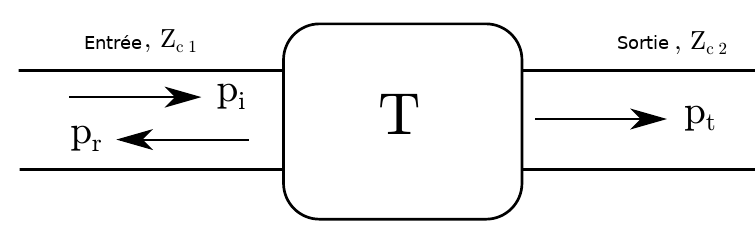
\includegraphics[ width=350px]{./images/th/scheme.png}
		\caption{Schéma matrice de transfert $T$ globale exprimé par la pression $p_1=p_i+p_r$ et $pt = p_2$}
		\label{schematrans}
	\end{figure}
	En combinant les équations \ref{eq:Tautrans2} et \ref{eq:Tglob} on peut écrire la transparence, donc l'indice d'affaiblissement depuis la matrice de transfert globale  (démonstration en annexe \ref{ch:demoafatrans}), dans le cas spécial d'air de chaque coté :
	\begin{equation}
	R = 20 \log_{10} \left\|T_{11}+\frac{T_{12}}{\rho_0 c_0}\cos\theta+\frac{\rho_0 c_0T_{21}}{\cos\theta}+T_{22}\right\|-6 \text{.}
	\end{equation}
	Sur les simulations effectuées, on retrouve les mêmes résultats avec la méthode des matrices de transferts que avec l'écriture du système complet. L'avantage de la méthode des matrices de transfert est qu'il permet de façon simple d'ajouter de l'amortissement, mais aussi de calculer le cas de plusieurs plaques.
	
	\section{Matériaux poreux : le modèle fluide équivalent}
	Les matériaux poreux sont une gamme de matériaux de traitement acoustiques utilisés pour l'absorption de large plages de fréquence, ceux-ci sont constitués d'une phase fluide (le plus souvent l'air) et d'une phase solide (le squelette de la mousse).\\
	Afin de prédire l'influence du matériau poreux utilisé, différents modèles ont été proposés, parmis les plus simples, on trouve le modèle empirique Delany-Bazley et le modèle Champoux-Allard-Johnson. Ceux ci permettent à partir des différents paramètres d'entrées des modèles de calculer l'impédance de surface du matériau $Z_p$ et sont nombre d'onde associé $k_p$.
	
	\subsection{Modèle Delany Bazley, Miki}
	Les travaux de \cite{delany_acoustical_1970}  ont été basé sur une campagne de mesure d'un nombre important de matériaux poreux. Suite à ces mesures, un modèle linéaire a été déduit. Ce modèle à l'avantage de ne nécessiter qu'un seul paramètre $\sigma$ pour modéliser la réponse du matériau, mais reste très limité dans sa validité fréquentielle et des paramètres du poreux. Plus tard, Miki utilise ces mêmes mesures  \cite{miki1990acoustical} pour créer un modèle amélioré. Les deux caractéristiques sont calculées avec :
	
	\begin{equation}
	Z_p = \rho_0 c_0 (1 + 0.070 (\frac{f}{\sigma})^{0.682}- 0.0107 U ^{-0.732}j),\text{.}
	\end{equation}
	
	\begin{equation}
	k_p = \frac{\omega}{c_0}(1 + 0.0978U^{-0.7}-  0.189U^{0.595}) \text{.}
	\end{equation}
	Avec 	$U$  défini par :
	\begin{equation}
	U=\frac{\rho_0 f}{\sigma} \text{,}
	\end{equation}
	où $\rho_0$ définie la densité de l'air, $c_0$ la célérité du son dans l'air, $\sigma$  la résistance au passage de l’air  et $\omega$ la fréquence angulaire. Unité en USI .\\
	
	Le modèle est valide pour une plage de fréquence particulière :
	\begin{equation}
	0.1 < U < 1.
	\end{equation}
	
	
	\subsection{Modèle Johnson-Allard-Champoux}
	Ce modèle est plus complexe est présenté dans le livre \cite{allard_propagation_2009} et prend en compte 5 paramètres. Il est valide pour une plus large bande de matériaux, cependant quand le squelette du matériau poreux est mis en vibration ce modèle n'est plus valide (matériaux à forte résistivité). Les différents caractéristiques:
	\begin{itemize}
		\item La tortuosité $\alpha_\infty$,caractérisant  le chemin de l'air dans un matériau poreux relatif au chemin direct.
		\item La porosité $\phi$, définie par le volume relatif entre le fluide d'air  et le volume total.
		\item La longueur caractéristique thermique $\lambda'$.
		\item La longueur caractéristique visqueuse $\lambda$.
		\item La résistance au passage de l'air $\sigma$. \\
	\end{itemize} 
	Afin de pouvoir calculer la l'impédance $Z_p$ et le nombre d'onde $k_p$, on calcule d'abord :
	\begin{itemize}
		\item la densité effective :
		\begin{equation}
		\rho_{eff} = \alpha(\omega) \rho_0.
		\label{eq:rhoeff}
		\end{equation}
		\item le module d'élasticité isostatique $K$ est donnée par :
		\begin{equation}
		K_{eff}= \frac{P_0}{\left(1- \frac{\gamma-1}{\gamma \alpha'(\omega)}\right)}
		\end{equation}
	\end{itemize}
	Le coefficient $\alpha(\omega)$, la tortuosité dynamique, à été donné dans un premier modèle par  \cite{johnson_theory_1987} :
	\begin{equation}
	\alpha(\omega) = \frac{\nu \phi }{j \omega q_0} \left[1 + \left(\frac{2\alpha_\infty q_0}{\phi \lambda}\right)^2 \frac{j \omega}{\nu} \right]^{1/2}+\alpha_\infty\text{.}
	\label{dtortue}
	\end{equation}
	Un coefficient $\alpha'(\omega)$ amélioré est donné dans \cite{champoux_dynamic_1991}, par l'équation: 
	\begin{equation}
	\alpha'(\omega)= \frac{8\nu'}{j \omega (\lambda')^2 }\left[ 1+ \left(\frac{\lambda'}{4}\right)^2 \frac{j \omega}{\nu'} \right]^{1/2}+1\text{.}
	\end{equation}
	
	Les coefficients finaux sont obtenus par :
	
	\begin{equation}
	Z_p= \sqrt{ \rho_{eff} K_{eff} } \text{.}
	\end{equation}
	\begin{equation}
	k_p=\omega \sqrt{ \frac{ \rho_{eff} }{ K_{eff} } } \text{.}
	\end{equation}
	
	\subsection{Comparaison des modèles}
	Les deux modèles sont présentés sur la Figure \ref{Zp}, représentant les impédances de surface et la Figure \ref{alphap} représentant le coefficient d'absorption posé sur un sol rigide. \\
	On voit que les deux modèles se rejoignent fortement, mais la méthode JAC sera retenu pour la suite, la bande de fréquence utile étant plus grande. \\ \\
	Les paramètres utilisés sont ceux d'une laine de roche trouvés dans un article sur internet, \cite{gle_acoustique_2013},ils sont donnés Table \ref{tab:porous}. Ils seront utilisés dans toutes les simulations suivante utilisant un matériau poreux.
	\begin{table}[h]
		\centering
		\begin{tabular}{|c|c|c|c|c|c|}
			\hline
			Épaisseur[cm] & $\sigma [kNs/m^4]$ & Porosité \% & Tortuosité  & $\lambda' [\mu m]$ & $\lambda [\mu m]$ \\ \hline
			10 & 20.6 & 98 & 1.01 & 90 & 85\\ \hline
		\end{tabular}
		\caption{JAC paramètres pour une laine de roche.}
		\label{tab:porous}
	\end{table}
	
	\begin{figure}[h]
		\begin{minipage}[c]{.45\linewidth}
			\begin{center}
				\makebox[0pt]{\includegraphics[width=300px]{images/th/Zp_mikjca.eps}}
				\caption{Impédance de surface d'une laine de roche, modèle de Miki et JAC.  \href{https://github.com/Nuopel/Encoffrement/blob/master/Programme/Comp_Champoux_Allard_Jonh.m}{Lien prog.}}
				\label{Zp}
			\end{center}
		\end{minipage}
		\hfill
		\begin{minipage}[c]{.45\linewidth}
			\begin{center}
				\makebox[0pt]{\includegraphics[width=300px]{images/th/absorptionmikjca.eps}}	
				\caption{Comparaison de l'affaiblissement mesuré  double et triple paroi.  \href{https://github.com/Nuopel/Encoffrement/blob/master/Programme/Comp_Champoux_Allard_Jonh.m}{Lien prog.}}
				\label{alphap}
			\end{center}
		\end{minipage}
	\end{figure}
	\section{Influence du matériau poreux}
	Le matériau poreux est une possibilité pour réduire l'influence des résonances sur l'indice d'affaiblissement. Afin de modéliser celui-ci, le modèle de Champoux-Allard-Johnson vu précédemment est utilisé, il permet d'obtenir une densité fluide équivalente $\rho_p$ avec l' Eq.\ref{eq:rhoeff} et le nombre d'onde équivalent $k_p$.
	\\ Bien que les paramètres utilisés (Tab \ref{tab:porous}) ne sont probablement pas exactement les mêmes que ceux de la laine de roche utilisée, ils peuvent servir de référence pour voir comment se comporte l'encoffrement avec amortissement.\\ \\
	Le cas étudié est un double encoffrement dont le milieu possède de la laine  de roche.
	En repartant des équations de continuités écrite plus haut, on peut écrire à nouveau les équations avec une densité $\rho_p$ et un nombre d'onde équivalent  $k_p$ pour le matériau poreux et écrire le système (Démonstration annexe \ref{ch:demoporeux}), en remplaçant $\cos \theta$ par $\Theta$ et $\cos \theta_p$ par $\Theta_p$ :
	\begin{align}	
	\begin{bmatrix}
	j k_0 \Theta    &0 & 0 &0&\rho_0\omega^2&0  \\
	0       & -j k_p \Theta_p & j k_p \Theta_p & 0 &\rho_p\omega^2 & 0  \\
	1       & -1 & -1 & 0 &-\mu \omega^2+Dk^4 & 0  \\
	0    &-j k_p \Theta_p e^{-jk_p\Theta_p e}   & j k_p \Theta_p e^{jk_p\Theta_p e}   &0&0&\rho_p\omega^2  \\
	0       & 0 & 0 &- j k_0 \Theta e^{-jk_0\Theta e} &0 & \rho_0\omega^2   \\
	0     & + e^{-jk_p\Theta_p e} & +e^{jk_p\Theta_p e} & - 	e^{-jk_0\Theta e} &0 & -\mu \omega^2+Dk^4  \\
	\end{bmatrix}
	\begin{Bmatrix}
	A_{ref} \\
	A_{tr2} \\
	A_{ref2}\\
	A_{tr3}\\
	C_{1} \\
	C_{2} 
	\end{Bmatrix}
	=\begin{Bmatrix}
	j k_0 \Theta \\
	0 \\
	-1\\
	0\\
	0 \\
	0
	\end{Bmatrix}
	\end{align}
	Le résultat pour  la même configuration que précédemment Figure \ref{w} avec la laine de roche est donné figure \ref{double+amo}, on voit qu'avec le matériau poreux (pointillés rouges) que l'affaiblissement augmente beaucoup plus en haute fréquences et la fréquence $f_r$ est repoussée vers le bas, de plus les pics liés aux ondes stationnaires sont disparus  . Bien que ce soit le résultat escompté, la disparition est totale, ce qui laisse planer un doute quand aux résultats. Ces résultats sont cependant comparés avec les résultats de la méthode MT (pointillés jaunes) où l'on voit que le résultat est confirmé.
	
	\begin{figure}[h!]
		\centering
		\includegraphics[ width=350px]{./images/th/compdoubleplaqueamortissement.eps}
		\caption{Comparaison de l'indice d'affaiblissement d'une plaque double avec et sans amortissement (même configuration que Figure \ref{w}). $\theta = 60\degres$, espacement 10 cm. Les fréquences de coïncidences sont notés par des traits rouges et les 5 premières fréquences d'ondes stationnaires en vert. \href{https://github.com/Nuopel/Encoffrement/blob/master/Programme/comparaison_cloison1_amortissement.m}{Lien prog.}}
		\label{double+amo}
	\end{figure}
	
	\section{Champ diffus}
	
	Pour l'étude de la transmission acoustique dans un champ diffus, on a d'après le cours \cite{cours}:
	\begin{equation}
	{\tau _d}(\omega ) = \frac{{\int_0^{2\pi } {\int_0^{\frac{\pi }{2}} {\tau (\omega ,\theta )\frac{{\cos \theta \sin \theta }}{{8\pi \rho c}}d\theta d\varphi } } }}{{\int_0^{2\pi } {\int_0^{\frac{\pi }{2}} {\frac{{\cos \theta \sin \theta }}{{8\pi \rho c}}d\theta d\varphi } } }}
	\end{equation}
	En simplifiant, on obtient:
	\begin{equation}
	{\tau _d}(\omega ) = 2\int_0^{\frac{\pi }{2}} {\tau (\omega ,\theta )\cos \theta \sin \theta d\theta }
	\end{equation}
	
	L'intégration numérique a été calculée avec Matlab en utilisant la commande \textit{matlabFunction} pour créé une fonction handle qui est ensuite évalué avec la commande \textit{integral} entre 0 et 60 degrée, considérant que dans une boite le champ direct n'a pas d'angle rasant. Un autre schéma d'intégration utilisant la commande \textit{int} évalué avec \textit{subs} a été testé mais était beaucoup plus long pour des performances qui semblaient similaires. \\
	La figure \ref{diffuscompall} présente les résultats comparant les solutions avec le système d'équations et les matrices de transfert pour les cloisons simples, doubles et triple.\\
	Pour le cas simple, on voit que les deux méthodes donnent le même résultat, la fréquence de coïncidence ne tombe plus à zéros. \\
	Pour le cas double , on voit que les deux méthodes donnent pratiquement le même résultat, excepté au niveau de la fréquence de respiration ($f_r$) où l'un fait un creux vers le haut et l'autre vers le bas, il serait plus logique que cela se déplace vers le bas, étant donné que $f_r$ se déplace avec l'angle et tend vers zéro, dans les deux cas le champ diffus améliore le phénomène défavorable de $f_r$. Ensuite on voit qu'un problème lors de l'intégration numérique apparaît à la fréquence critique la plus faible des deux plaques pour les MT, où les résultats chutent inexplicablement et oscillent beaucoup, l'autre méthode semble aller un peu plus loin en fréquence avant d'avoir le même problème.\\
	Pour le cas triple , on voit que les deux méthodes ne donnent pas du tout le même résultat il y a un écart qui n'est pas expliqué, puis à partir de la même fréquence que pour les doubles plaques, le schéma numérique explose. D'un point de vue global on observe que le cas triple marche mieux que le cas double et simple.\\ 
	
	La figure \ref{diffuscompporeux} présente les résultats en champ diffus de cloison double et triple, en comparant le cas avec amortissement (poreux + amortissement plaque) et sans matériau poreux. On voit que l'amortissement améliore grandement les performances dans les deux cas.
	
	On note aussi que la cloison ajoute un léger avantage d'amortissement en champ diffus. En effet, l'indice d'affaiblissement a tendance à légèrement augmenter en présence d'amortissement de la cloison aux fréquences supérieures à la fréquence critique. \\
	\begin{figure}[h]
		\begin{minipage}[c]{.45\linewidth}
			\begin{center}
				\makebox[0pt]{\includegraphics[width=300px]{images/th/diffuscomp_all.eps}}
				\caption{Champ diffus avec les deux méthodes, simple, double et triple plaques avec les paramètres Tab.\ref{tab:paraplaques}, espacement 1 = 10cm, espacement 2 = 8cm. \href{https://github.com/Nuopel/Encoffrement/blob/master/Programme/Champ_diffu.m}{Lien prog}}
				\label{diffuscompall}
			\end{center}
		\end{minipage}
		\hfill
		\begin{minipage}[c]{.45\linewidth}
			\begin{center}
				\makebox[0pt]{\includegraphics[width=300px]{images/opt/R_diffus_compdt.eps}}	
				\caption{Champ diffus avec la méthode matrice de tranfert, double et triple, cas poreux et non poreux, plaques avec les paramètres Tab. \ref{tab:paraplaques}, espacement 1 = 10cm, espacement 2 = 8cm.\href{https://github.com/Nuopel/Encoffrement/blob/master/Programme/Champ_diffu_TransMat.m}{Lien prog.}} 
				\label{diffuscompporeux}
			\end{center}
		\end{minipage}
	\end{figure}
	
	\section{Un modèle fini plus réaliste}
	
	L'aspect fini de la cloison agit aussi sur l'indice d'affaiblissement. Afin de voir quel serait cette effet la Thèse de master basé sur l'article de \cite{villot_predicting_2001} propose de calculer la transmission acoustique $\tau$ à partir d'un facteur de correction sur le $\tau_{inf}$ infini.\\
	En prenant une plaque finie de dimension $a$ et $b$, la transmission peut être obtenue en appliquant un fenêtrage spatial selon l'équation :
	\begin{equation}
	\tau  = \frac{\sigma }{{{\sigma _{\inf }}}}{\tau _{\inf }} \text{,}
	\label{eq:pfini}\end{equation}
	où ${\sigma _{\inf }} = \frac{1}{{\cos \theta }}$ et $\sigma$ est l'efficacité de rayonnement de la plaque finie.\\
	On peut alors écrire de manière simplifiée, en prenant en compte la longueur définie par $L = \sqrt {ab} $ l'Eq. \ref{eq:pfini} qui amène une double correction associée à chacune des longueurs:
	\begin{equation}
	\tau (f,\theta ) = {\tau _{\inf }}(f,\theta ){\left( {\sigma (f,\theta )\cos \theta )} \right)^2} \text{,}
	\end{equation}
	L'efficacité de rayonnement peut être calculée avec : \\
	\begin{equation}
	\sigma ({k_p}) = \frac{{L{k_a}}}{{2\pi }}\int_0^{{k_a}} {\frac{{{{\sin }^2}\left[ {({k_r} - {k_p})\frac{L}{2}} \right]}}{{{{\left[ {({k_r} - {k_p})\frac{L}{2}} \right]}^2}\sqrt {k_a^2 - k_r^2} }}d{k_r}}\text{.}
	\end{equation} \\
	Cette équation n'est valable que pour les plaques avec ratio de dimension inférieur à 1:2.
	où $k_a$ est le nombre d'onde de l'air et $k_p$ le nombre d'onde de la plaque.\\
	La Figure \ref{fini1} présente les résultats de cette méthode pour une plaque finie comparé à une plaque infinie, on voit qu'en haute fréquence le comportement est le même alors qu'en basse fréquence l'indice d'affaiblissement augmente, ceci est due à l'efficacité de rayonnement $\sigma$ présenté Fig. \ref{finisig} qui tend vers 1 après la fréquence critique de la plaque, tout comme la plaque infinie. On voit cependant que les résultats basse fréquence semble beaucoup trop bon, et remettent en question la validité des résultats. Le comportement de $\sigma$  est confirmé par plusieurs sources \cite{allard_propagation_2009},\cite{villot_predicting_2001}. La formule \ref{eq:pfini} ne fait pas tendre l'affaiblissement vers une réponse infinie quand on augmente la taille car  $\sigma$ dans le cas infini est plus faible que dans le cas fini (Fig. \ref{finisig}).\\ Par manque de temps, l'investigation ne fût pas poussé plus loin. \\
	Cependant il semble bien que l'aspect fini des plaques augmente les performances de l'indice d'affaiblissement comme le montre les résultats dans \cite{villot_predicting_2001} (exemple dans les figures 14-16 de l'article).
	
	\begin{figure}[h]
		\begin{minipage}[c]{.45\linewidth}
			\begin{center}
				\makebox[0pt]{\includegraphics[width=300px]{images/th/finiR.eps}}
				\caption{Indice d'affaiblissement avec filtrage spatial pour une plaque 0.4m x 0.4m, possédant les propriétés de la première ligne Tab. \ref{tab:paraplaques} et un $\theta=40\degres$.\href{https://github.com/Nuopel/Encoffrement/blob/master/Programme/simplecloison_finite_size.m}{Lien prog.}}
				\label{fini1}
			\end{center}
		\end{minipage}
		\hfill
		\begin{minipage}[c]{.45\linewidth}
			\begin{center}
				\makebox[0pt]{\includegraphics[width=300px]{images/th/sigma.eps}}	
				\caption{Efficacité de rayonnement associé à la plaque 0.4m x 0.4m et infini possédant les propriétés de la première ligne Tab\ref{tab:paraplaques}.\href{https://github.com/Nuopel/Encoffrement/blob/master/Programme/simplecloison_finite_size.m}{Lien prog.}}
				\label{finisig}
			\end{center}
		\end{minipage}
	\end{figure}
	\section{Influence de l'encoffrement: ajout du champ réverbéré}
	Pour passer de l'étude d'une plaque vers un encoffrement, il faudra donc tenir compte de l'effet de réverbération du champ diffus créé par les réflexions des ondes sur les parois de l'encoffrement.
	Celui-ci dépend de l'absorption totale de la paroi et de la source et est présenté dans \cite{vas}. 
	
	On aura tout d'abord un rayonnement direct venant de la source et entre en contact avec la paroi juste avant la première réflexion. La puissance acoustique transmise à ce niveau sera le produit de la puissance incidente \textit{W} et le coefficient de transmission moyen \({\tau _0}\) de la cloison pour des ondes en incidence normale.
	\begin{align}
	\begin{cases}
	W_{TD} = W{\tau _0} \\
	\tau _0 = 0.316\tau  \text{,}
	\end{cases}
	\end{align}
	
	avec \({W_{TD}}\) la puissance transmise directe et \({\tau}\) le coefficient de transmission en champ diffus.\\
	
	Après réflexion des ondes et absorption partielle au niveau de la paroi par le matériau poreux, on aura une puissance réfléchie qui va encore affecter le champ réverbéré dans l'encoffrement. Cette puissance peut être calculée à partir de la puissance acoustique en incidence directe et du coefficient d'absorption moyen \(\bar \alpha \) à l'intérieur de l'encoffrement  .
	\begin{equation}
	W_R = W_{TD}(1 - \bar \alpha )\text{.}
	\end{equation}
	Le modèle de Sabine nous servira à déterminer donc le niveau de pression acoustique du champ réverbéré selon la formule suivante:
	\begin{equation}
	\frac{{p_R^2}}{{\rho c}} = \frac{{4{W_R}}}{A}\text{,}
	\end{equation}
	avec \textit{A} l'aire d'absorption du volume intérieur qui est aussi calculée par:
	\begin{equation}
	A = \bar \alpha {S_i}\text{,}
	\end{equation}
	où \({S_i}\)  est la surface totale intérieure de l'encoffrement.
	
	On peut ensuite déterminer le flux de puissance incident sur les parois du au champ réverbéré par:
	\begin{equation}
	{W_{inc}} = \frac{{\left\langle {p_R^2} \right\rangle }}{{\rho c}}S = \frac{{{W_R}S}}{A} = \frac{{W_{TD}(1 - \bar \alpha )S}}{{\bar \alpha {S_i}}}\text{.}
	\end{equation}
	Finalement la puissance transmise après effet de réverbération est donnée par:
	\begin{equation}
	{W_{TR}} = {W_{inc}}\tau \text{.}
	\end{equation}
	
	La puissance totale transmise est la somme de celle transmise en champ direct \(W_{TD}\) et en champ réverbéré \(W_{TR}\).
	\begin{equation}
	{W_T} = 0.3\tau W + \tau \frac{{W(1 - \bar \alpha )S}}{{\bar \alpha {S_i}}}\text{.}
	\end{equation}
	
	On peut donc obtenir la perte par insertion:
	\begin{equation}
	D = 10\log \frac{W}{{{W_T}}} = 10\log \frac{1}{\tau } - 10\log (0.3 + \frac{{1 - \bar \alpha }}{{\bar \alpha }}\frac{S}{{{S_i}}})\text{.}
	\end{equation}
	Dans la suite de cette étude, on ne tiendra pas en compte l'influence du champ réverbéré pour simplifier le modèle, mais l'on s'attend à se que cela baisse les performances en basse fréquence à cause du ratio $\frac{\tilde{\alpha}}{1-\tilde{\alpha}}$ qui augmente quand $\alpha$ diminue (basse fréquence).
	
	\chapter{Simulations, optimisation et construction du prototype}
	
	Les paramètres des plaques étudiées dans cette étude sont résumés dans le tableau suivant:
	
	\begin{table}[h]
		\centering
		\begin{tabular}{|c|c|c|c|c|}
			\hline
			Plaques[MDF]& Épaisseur [mm]& Module d'Young [GPa]& Densité $[Kg/m^3] $& $\nu$ Coefficient de Poisson  \\ \hline
			Plaque 1 & 1.3 & 2.3 & 750 & 0.245 \\ \hline
			Plaque 2 & 6.4 & 3 & 750 & 0.245\\ \hline
			Plaque 3 & 12.7 & 3 & 750 & 0.245\\ \hline
		\end{tabular}
		\caption{Paramètres des les plaques de MDF étudiées.}
		\label{tab:paraplaques}
	\end{table}
	
	Le code Matlab \href{https://github.com/Nuopel/Encoffrement/blob/master/Programme/comparaison_cloison_amortissement_TransMat.m}{(lien prog)} sert à étudier les comportements de ces plaques MDF sur une gamme de fréquence de 0 à 11 KHz pour nous aider à faire le choix de la configuration finale à utiliser pour l'encoffrement.\\
	L'avantage évident de la double cloison dans les précédents chapitres sur la simple cloison fait que l'on ne parlera que des doubles et triples cloisons.\\ Il a été observé dans les simulations que le fait de choisir des plaques aux propriétés différentes permet d'éviter que les fréquences de coïncidences ne soit aux mêmes endroits et diminuent les performances. Il en va de même pour les fréquences de résonances demi-ondes, bien que grandement limités par la présence de matériaux poreux.\\ L'effet cavité n'est pas représenté dans les simulations, il est cependant attendu que celle ci joue un rôle défavorable, le fait d'avoir des dimensions identiques risquent probablement d'amplifier les phénomènes défavorables aux mêmes fréquences, dans la mesure du possible, nous essaierons d'avoir des dimensions différentes.\\
	Enfin la masse joue un grand rôle dans l'atténuation, directement lié à l'épaisseur. En considérant l'encoffrement comme des plaques infinies repliés autour de la source, on choisira donc de mettre les épaisseurs dans un ordre croissant afin que la source soit entourée par la plaque la plus épaisse. Ainsi pour une même performance idéale, on diminuera le poids de l'encoffrement dans la réalité.\\
	
	Les impératifs de constructions et d'accessibilités des matériaux ont porté les choix entre du MDF et du contre-plaqué, les performances du premier type était plus importante, probablement due au fait que la densité était plus élevée. Au final les contraintes techniques et budgétaires nous on fait porté le choix sur les plaques aux paramètres Tab. \ref{tab:paraplaques}.\\
	La figure \ref{comp3_0} illustre les résultats des configurations étudiées à un angle de 0 degrée, tandis que la Figure \ref{comp3_50} est à 50 degrée. On voit que les deux premières plaques en double encoffrement (courbe jaune) isole mieux le bruit que les deux dernières plaques (courbe violette). Ceci est du à l'épaisseur des plaques prises en compte. En effet elles sont plus épaisses que les deux dernières (1/4" \& 1/2" vs 1/2" \& 1/8"). Si l'on compare ces résultats à la triple cloison sans amortissement  on voit qu'il n' y a pas une si grande différence au niveau de l'amplitude de l'indice d'affaiblissement au milieu de la courbe, en basse fréquence cependant on observe que les fréquences de respirations donnent de moins bon résultats. En haute fréquence l'avantage est flagrant. Si l'on compare les résultats avec amortissement, on voit alors que la triple cloison à la même réponse en basse fréquence, l'amortissement lisse la courbe, mais une réponse bien supérieure après.\\
	On pourrait se demander à épaisseur équivalente totale et espace équivalent total entre une configuration triple et double si les performances seraient toujours meilleures. Ce cas est montré Figure \ref{compeq}, où l'on a la même triple cloison qu'avant et une double cloison dont l'espacement est la somme des deux espaces de la triple et où la somme de l'épaisseur des deux plaques est égale à celle de la triple (7/8" et 5/8"). On voit que en basse fréquence les performances sont moins bonne avec la triple mais que en haute fréquence elles sont meilleures. En ajoutant la masse et une réalisation physique en considération, on déduit cependant qu'une configuration triple reste plus légère (car on aurait une très grande boite épaisse pour la double plutôt qu'une moyenne et une fine grande boite), donc plus performante.\\ \\
	
	
	\begin{figure}[h]
		\begin{minipage}[c]{.45\linewidth}
			\begin{center}
				\makebox[0pt]{\includegraphics[width=300px]{images/opt/comp32_0d.eps}}
				\caption{Indice d'affaiblissement d'une triple cloison avec et sans amortissement comparé aux deux doubles cloisons qui la compose, avec et sans amortissement pour un angle d'incidence de 0 \degres. possédant les propriétés du  Tab. \ref{tab:paraplaques}.\href{https://github.com/Nuopel/Encoffrement/blob/master/Programme/comparaison_cloison_amortissement_TransMat.m}{Lien prog.}}
				\label{comp3_0}
			\end{center}
		\end{minipage}
		\hfill
		\begin{minipage}[c]{.45\linewidth}
			\begin{center}
				\makebox[0pt]{\includegraphics[width=300px]{images/opt/comp32_50d.eps}}	
				\caption{Indice d'affaiblissement d'une triple cloison avec et sans amortissement comparé aux deux doubles cloisons qui la compose, avec et sans amortissement,les fréquences de coïncidences des 3 plaques sont notés par un trait rouge, pour un angle d'incidence de 50 \degres possédant les propriétés du Tab.\ref{tab:paraplaques}.\href{https://github.com/Nuopel/Encoffrement/blob/master/Programme/comparaison_cloison_amortissement_TransMat.m}{Lien prog.}}
				\label{comp3_50}
			\end{center}
		\end{minipage}
	\end{figure}
	Enfin la Fig.\ref{compoptdiffus}, présente le cas du champ diffus,
	Il n'y a pas de grandes différences de niveau d'indice d'affaiblissement de la triple cloison sans amortissement et ceux des doubles cloisons en basse fréquence. Par la suite, les résultats sont d'abord meilleurs avec la double puis largement meilleurs avec la triple.\\ 
	Le matériau absorbant ajoute un grand avantage d'affaiblissement à la triple cloison et semble limiter les erreurs d'intégrations numériques (les effets des ondes stationnaires qu'on retrouve dans la courbe de l'indice d'affaiblissement de la triple cloison sans amortissement?).\\ 
	En champ diffus, on évitera d'avoir des fréquences nulles au niveaux des fréquences de respirations et des éventuelles ondes stationnaires, ce qui avantagerait notre système d'isolation, bien qu'elles semblent lissés par l'amortissement. \\
	Selon les résultats présentés en champ diffus la configuration de triple cloison est sans doute la meilleure pour isoler le bruit car elle présente beaucoup plus d'avantages que les autres configurations.\\
	
	Les résultats d'indice d'affaiblissement trouvées semblent normaux jusqu'à 1200 Hz autour de la première fréquence critique, où le problème d'intégration numérique rend les résultats obtenus pas assez clairs pour être analysés.\\
	Malgré la perte de performance en masse qui subviendra, la triple cloison a donc été choisie comme configuration finale pour la fabrication de l'encoffrement. Les paramètres des plaques utilisés sont mis dans le Tableau \ref{tab:paraplaques} et la verre de roche dans le tableau \ref{tab:porous}.
	
	\begin{figure}[h]
		\begin{minipage}[c]{.45\linewidth}
			\begin{center}
				\makebox[0pt]{\includegraphics[width=300px]{images/opt/compeq.eps}}
				\caption{Indice d'affaiblissement d'une triple cloison avec et sans amortissement comparé à une double cloison d'espace et épaisseur équivalente.\href{https://github.com/Nuopel/Encoffrement/blob/master/Programme/comptriple_double_equivalente.m}{Lien Prog.}}
				\label{compeq}
			\end{center}
		\end{minipage}
		\hfill
		\begin{minipage}[c]{.45\linewidth}
			\begin{center}
				\makebox[0pt]{\includegraphics[width=300px]{images/opt/R_diffus_compdt.eps}}
				\caption{ Indice d’affaiblissement d’une double cloison avec et sans amortissement comparé à une triple cloison avec et sans amortissement en champ diffus. \href{https://github.com/Nuopel/Encoffrement/blob/master/Programme/Champ_diffu_TransMat.m}{Lien prog.}}
				\label{compoptdiffus}
			\end{center}
		\end{minipage}
	\end{figure}
	
	\section{Construction du prototype}
	
	Après avoir choisi la configuration finale en fonction des matériaux nécessaires pour l'encoffrement, du budget et des simulations, la laine de roche a été choisie comme matériau poreux, et des plaques MDF de différentes épaisseurs pour les plaques.\\
	L'épaisseur de laine de roche varie dans chaque espace entre les plaques comme le montre la Figure \ref{espacement_cloison} suivante : \\ \\
	
	\begin{figure}[h!]
		\centering
		\makebox[0pt]{\includegraphics[width=300px]{images/obj/Epaisseurs_Laine_de_roche.JPG}}
		\caption{Espacements entre les cloisons utilisé pour la fabrication de l'encoffrement.}
		\label{espacement_cloison}
	\end{figure}
	
	Le fait d'utiliser des plaques à tailles différentes nous aiderait à réduire les effets de mode de cavité des plaques mais pendant la construction, on a du minimiser l'espacement entre le haut-parleur et le premier cube pour réduire la masse totale. Après avoir ajouté les espacements entre les plaques, on s'est retrouvé avec une boite presque carrée (car on ajoute quasiment le même espacement à chaque dimension).\\
	
	\textbf{Dimensions}:
	\begin{itemize}
		\item  Le premier cube contenant le haut-parleur est de: 20 cm x 22 cm x 25 cm (LxPxH).
		\item Le cube du milieu a une dimension de : 42 cm x 44 cm x 46 cm (LxPxH). 
		\item Le plus grand cube contenant les deux autres a une dimension de: 60 cm x 60 cm x 60 cm (LxPxH). 
	\end{itemize}

	
	Afin d'empêcher les fuites, un joint de silicone a été utilisé au niveau de chaque bord des plaques. Des vis ont également été utilisés pour joindre les plaques et former des cubes.\\ 
	Afin de pondérer comme demandé dans le cahier des charges il est nécessaire de peser l'encoffrement, les masses de l'encoffrement sont :
	\begin{itemize}
		\item 16.86 Kg pour les deux cubes internes (double cloison incluant le matériau absorbant).
		\item 32.54 Kg pour l'encoffrement total (triple cloison incluant le matériau absorbant).
	\end{itemize}
	
	
	
	
	\chapter{Étude expérimentale et résultats}
	Le programme est disponible sur Github à l'adresse suivante :\\
	\href{https://github.com/Nuopel/Encoffrement/tree/master/Mesures\%20encoffrements-20170818}{https://github.com/Nuopel/Encoffrement/tree/master/Mesures\%20encoffrements-20170818}. Pour utiliser le programme "analyse\_meas.m" il faut télécharger les fichiers textes correspondant dans le même dossier.
	\section{Résultats expérimentaux \& Théoriques}
	Le test a été fait sur une plage de fréquence de 0Hz à 5kHz et le niveau de pression a été évalué dans la configuration présenté dans le  la section \ref{sec:critereeval} du chapitre \ref{ch:objectif}. \\
	Les résultats ont été données dans des fichiers Excel pour le post-traitement des données. expérimentales.\\
	Les $IL(w)$ par tiers d'octaves des configurations double (3/4" et 1/2") et triple couches sont comparés Figure \ref{compmeas}, les $IL$ globaux et pondérés sont marqués dans la légende et rappelés dans le tableau \ref{tab:resultatsIL}. \\
	
	La perte par insertion est supérieure dans le cas de la triple cloison, on trouve une différence de 13 dB entre les deux configurations. On le voit bien dans la figure \ref{compmeas}, où dans les fréquences médium la performance de la  triple couche est meilleure, tandis de en basse fréquence et en haute fréquence les deux résultat se rejoignent.\\
	Les indicateurs de de performance permettent de conclure que l'encoffrement de triple cloison est plus performante que la double sur une fréquence de 100 Hz à 5000 Hz dans le cas des systèmes utilisés pour mener cette étude.\\
	
	Dans les Figures \ref{compmeasthdouble} et \ref{compmeasthtriple} on compare les $IL(\omega)$ mesurés aux simulations en champ diffus avec et sans matériaux poreux.\\
	Les résultats d'indices d'affaiblissements obtenus en haute fréquence pour les simulations sont plus forts en amplitudes que ceux des expériences qui atteignent une limite. En basse fréquence, on observe une remontée de $IL(\omega)$ par rapport aux simulations qui ne font qu'augmenter de manière générale avec la fréquence. 
	
	\begin{figure}[h]
		\begin{center}
			\makebox[0pt]{\includegraphics[width=300px]{images/result/comp_rslt_td.eps}}
			\caption{Comparaison de l'affaiblissement mesuré double et triple paroi. \href{https://github.com/Nuopel/Encoffrement/blob/master/Mesures\%20encoffrements-20170818/analyse_meas.m}{lien prog.}  }
			\label{compmeas}
		\end{center}
	\end{figure}
	\begin{figure}[h]
		\begin{minipage}[c]{.45\linewidth}
			\begin{center}
				\makebox[0pt]{\includegraphics[width=300px]{images/result/comp_rslt_d_th.eps}}
				\caption{Comparaison de l'affaiblissement mesuré et simulé diffus double (avec et sans poreux). \href{https://github.com/Nuopel/Encoffrement/blob/master/Mesures\%20encoffrements-20170818/analyse_meas.m}{lien prog.}    }
				\label{compmeasthdouble}
			\end{center}
		\end{minipage}
		\hfill
		\begin{minipage}[c]{.45\linewidth}
			\begin{center}
				\makebox[0pt]{\includegraphics[width=300px]{images/result/comp_rslt_t_th.eps}}
				\caption{Comparaison de l'affaiblissement mesuré et simulé diffus triple   (avec et sans poreux).  \href{https://github.com/Nuopel/Encoffrement/blob/master/Mesures\%20encoffrements-20170818/analyse_meas.m}{lien prog.}  }
				\label{compmeasthtriple}
			\end{center}
		\end{minipage}
	\end{figure}
	
	
	La perte par insertion globale $IL_G$ et l'indicateur de performance $IL_M$ ont été calculés pour la double cloison et la triple cloison dans le tableau \ref{tab:resultatsIL} ci-dessous: \\
	\begin{table}[h!]
		\centering
		\begin{tabular}{|c|c|c|c|c|c|c|}
			\hline
			Configuration& Masse [Kg]& Perte par insertion globale $IL_G$ [dB]& Indicateur de performance $IL_M$ [dB]\\ \hline
			Cloison double & 16.86 & 45.3 & 20.7 \\ \hline
			Cloison triple & 32.54 & 58.3 & 28.1 \\ \hline
		\end{tabular}
		\caption{Résultats de pertes par insertion et indice de performance de chaque configuration.}
		\label{tab:resultatsIL}
	\end{table}
	
	
	
	\subsection{Discussion des différences théoriques et expérimentales}
	Les différences entre les résultats théoriques et expérimentaux peuvent être dues aux approximations et hypothèses prises en considérations lors de la modélisation (hypothèses de plaques finies, approximations numériques), mais aussi par les conditions expérimentales et la fabrication de la boite.\\
	
	\textbf{Approximations théoriques:}\\
	\begin{itemize}[label=\textbullet]
		\item Le haut-parleur a été considéré comme une source omnidirectionnelle, alors qu'en réalité il a une directivité particulière. Selon cette hypothèse, les pressions mesurées par tous les microphones devraient être les mêmes, mais ce n'est pas le cas dans les résultats expérimentaux. De plus le haut parleur est contenu dans une enceintfoe, ce qui en fait une source bafflée . \\ 
		\item L'influence des cavités n'a pas été prises en compte dans le modèle théorique utilisée.\\ 
		\item Les simulations ne prennent en compte que des plaques infinies, or il a été montré dans l'article de \cite{villot_predicting_2001} que les plaques finies augmente $IL$ en basse fréquence, ce qui pourrait expliquer pourquoi dans les mesures l'$IL$ ré-augmente (flagrant dans le cas double cloison).\\
		\item Le matériau absorbant a été pris en compte en utilisant le modèle de Johnson-Allard-Champoux qui n'est valable qu'en utilisant certaines hypothèses d'épaisseurs et de résistivité. Toutefois pour la réalisation, la laine roche utilisé pourrait ne pas correspondre parfaitement à celle de la simulation.\\
	\end{itemize}
	
	\textbf{Incertitudes liés à la construction physique}\\
	\begin{itemize}[label=\textbullet]
		\item Des fuites acoustiques peuvent être à l'origine d'une dégradation de la performance de l'encoffrement car des trous ont été percés pour chaque cube  afin de laisser passer les fils (même si on a essayé de mettre du mastique). Des fuites sont aussi présentes à cause de la façon de joindre les plaques en forme de cube avec des vis, nous avons mis du joint sur les arrêtes mais nous n'avons pas pus en mettre sur le socle fermant. Ces fuites jouent surtout sur les basses fréquences. \\ 
		\item Les paramètres de plaques utilisés pour la fabrications sont incertains, les vraies valeurs de densité, de coefficient de Poisson, de module d'Young et de résistivité  ne sont pas donnés par l'endroit où nous les avons achetés. Elle peuvent être différentes des valeurs prises durant les simulations qui ont été prises sur internet.\\
	\end{itemize}
	
	\textbf{ Incertitudes expérimentales:}\\
	\begin{itemize}[label=\textbullet]
		\item La source possède une réponse en fréquence non plate, comme nos mesures sont réalisées entre 20Hz et 5000Hz, cela ne jouera que sur les basses fréquences où le haut parleur n'arrive pas à fournir d'énergie, il est donc normal que plus l'on arrive près de 0 Hz plus le coefficient diminue car on ne mesure plus que le bruit de fond avec et sans boite. Il est à noté que cela n'est pas pris en compte dans les $IL$ globaux qui sont calculés entre 100Hz et 5000Hz. \\
		\item Le bruit de fond se confond avec les résultats en haute fréquence, les encoffrements amortissent trop pour être mesuré. Cela est visible dans la figure \ref{compmeas} où à partir d'un $IL$ de 50dB les courbes deviennent pratiquement plates, il est aussi possible que cette limite dépende de la fréquence.\\
		\item   Pendant le test, les microphones n'ont pas été calibrés les uns par rapport aux autres, ils pourraient donc avoir des sensibilités différentes qui ne sont pas pris en compte dans le rapport des sommes des pressions. \\ 
	\end{itemize}
	
	
	\chapter{Conclusion}
	
	Cette étude avait pour but de créer un encoffrement qui aurait un $IL$ minimum de 15 dB sur la plage de fréquence prévu dans le cahier des charges (100Hz-10kHz).
	
	Afin d'achever ce résultat nous avons d'abord réalisé une approche théorique.\\ Nous sommes partis de l'hypothèse que l'encoffrement pouvait être assimilé à une plaque infinie comme vue dans le cours. Le modèle à ensuite été complexifié en utilisant une double cloison fondé sur les notions du devoir 6, puis par extension une triple cloison. Une comparaison de ces résultats à été fait avec la méthode des matrices de transfert qui se révèle beaucoup plus simple à implémenter (la compréhension physique est néanmoins plus claire avec la méthode du cours ). Un modèle de matériau poreux à été ajouté à nos calcul afin de palier aux résonances qui dégradaient les résultats. Enfin des calculs de champ diffus ont été réalisés pour se rapprocher plus de la réalité, avec la limitation que des erreurs d'intégrations numériques apparaissaient dans les résultats, les rendants difficiles à exploiter.\\
	
	Ensuite plusieurs considérations  physiques ont été vues pour voir quel seraient leurs effets dans la réalité: l'effet du champ réverbéré et l'impact de la dimension finie de la plaque.
	
	Le budget maximum et la performance désirée a été une limite pour le choix des matériaux et de la configuration à utiliser.\\
	Grâce à l'approche théorique un modèle Matlab a été développé en se limitant aux matériaux possibles à utiliser pour la réalisation.\\
	Le MDF et la laine de roche ont finalement été retenus  pour la construction de cet encoffrement et un triple encoffrement à été retenu.\\
	
	L'indicateur de performance final obtenu pour la configuration triple paroi est de 28.1 dB qui est largement supérieur à l'objectif visé.\\
	Les résultats expérimentaux ont servi à discuter du modèle considéré pour l'étude et proposer des corrections aux considérations prises plus tôt dans la simulation pour obtenir une meilleure performance. On a pu observer que les écarts entre les résultats théoriques et expérimentaux sont un peu larges. Ces différences pourraient être réduites lors d'une prochaine étude en tenant compte des facteurs énumérés plus haut. Une autre façon d'améliorer les performances serait d'utiliser des résonnateurs de Helmholtz(qui n'a pas été traité) et de réussir à d'utiliser le modèle de fenêtrage spatial de plaques finies.\\
	
	Pour finir,le choix des matériaux et de leurs dispositions à joué un rôle primordial pour atteindre l'objectif fixé. Le budget, l'accessibilité aux matériaux et leurs usinages définissait le choix des matériaux, on a été contraint à une courte liste de choix. Le modèle théorique n'a donc servit qu'à prédire les résultats d'isolation des quelques choix possibles plutôt qu'une vraie optimisation.\\
	
	\printbibliography
	\appendix
	\chapter{Démonstration plaque double devoir 6 GMC721}
	\label{ch:demodev6}
	\subsection*{Équations acoustique}
	À partir de considérations physiques on peut directement établir les équations des pressions acoustiques dans chacun des milieux. En effet, en assumant une onde plane arrivant sur une plaque infinie on se retrouve avec des solutions d'ondes planes. Les ondes planes étant solutions de l'équation d'onde on a un schéma de propagation acoustique valide.\\ 
	À chaque interface il y a des ondes transmises et des ondes réfléchies, la somme de ces ondes est réduite à une onde transmise et une onde réfléchie.\\ \\
	Les pressions dans les différents milieux sont donc : était
	\begin{align}
	\textbf{milieu 1 :} &
	\begin{cases}
	P_{1,1} &= A_{inc}e^{jwt-jk\cos\theta x_1-jk_1\sin\theta x_3} \text{, la pression incidente}\\
	P_{1,2} &= A_{ref}e^{jwt+jk_1\cos\theta x_1-jk_1\sin\theta x_3}\text{, la pression réfléchie}\\
	\end{cases}\\
	\textbf{milieu 2 :} &
	\begin{cases}
	P_{2,1} &= A_{tr2}e^{jwt-jk_2\cos\theta_2 x_1-jk_2\sin\theta_2 x_3} \text{, la pression transmise}\\
	P_{2,2} &= A_{ref2}e^{jwt+jk_2\cos\theta_2 x_1-jk_2\sin\theta_2 x_3}\text{, la pression réfléchie}\\
	\end{cases}\\
	\textbf{milieu 3 :} &
	\begin{cases}
	P_{3} &= A_{3}e^{jwt-jk_3\cos\theta_3 x_1-jk_3\sin\theta_3 x_3} \text{, la pression transmise.}
	\end{cases}
	\end{align}\\
	Par soucis de simplicité, les $e^{jwt}$ seront omis dans les écritures et $A_{inc}=1$.
	\subsection*{Équations mécanique}
	L'équation d'une plaque est donné par : 	
	\begin{equation}
	\mu \frac{\partial^2w}{\partial t^2}+D\triangle^4w = p_- -p_+
	\end{equation}
	Les solutions de cette équation pour une plaque infinie sont : 
	\begin{align}
	\begin{cases}
	w_p &= Ce^{-jwt-jkx_3} \text{, la solution propagative}\\
	w_e &= Ce^{-jwt-kx_3}\text{, la solution évanescente,}\\
	\end{cases}
	\end{align}
	Donc les équations aux deux plaques identiques sont : 
	\begin{align}
	\begin{cases}
	w_{p1} &= C_{p1}e^{-jwt-jkx_3} \text{, la solution propagative}\\
	w_{e1} &= C_{e1}^{-jwt-kx_3}\text{, la solution évanescente}\\
	\end{cases}\\
	\begin{cases}
	w_{p2} &= C_{p2}e^{-jwt-jkx_3} \text{, la solution propagative}\\
	w_{e2} &= C_{e2}^{-jwt-kx_3}\text{, la solution évanescente,}\\
	\end{cases}
	\end{align}
	Cependant considérant la plaque excité par des ondes acoustiques, les ondes de la plaque seront toujours supersoniques, les solutions évanescentes n'étant pas physiques on a :
	\begin{align}
	\begin{cases}
	w_{1} &= C_{1}e^{-jwt-jk_{p1}x_3} \text{, la solution propagative plaque 1}\\
	w_{2} &= C_{2}e^{-jwt-jk_{p2}x_3} \text{, la solution propagative plaque 2}\\
	\end{cases}
	\end{align}
	\textbf{Remarque:} $k_{p1}$ et $k_{p2}$ sont différent du nombre d'onde associé à l'équation de dispersion de la plaque et sont imposés par l'onde acoustique.
	\subsection*{Équations de continuités}
	Les équations de continuités sont : 
	\begin{align}
	\textbf{ plaque 1}&\begin{cases}
	\frac{\partial P_{1,1}}{\partial x_1}+\frac{\partial P_{1,2}}{\partial x_1} = \rho_0\omega^2w_1(x_3,t)\text{ à }x_1=0\\
	\frac{\partial P_{2,1}}{\partial x_1}+\frac{\partial P_{2,2}}{\partial x_1}  = \rho_0 \omega^2 w_1(x_3,t)\text{ à }x_1=0\\
	-\mu_1 \omega^2w_1+D_1\nabla^4w_1 = P_{1,1}+P_{1,2}-P_{2,1}-P_{2,2} \text{ à }x_1=0\text{.}
	\end{cases}\\
	\textbf{ plaque 2}&\begin{cases}
	\frac{\partial P_{2,1}}{\partial x_1}+\frac{\partial P_{2,2}}{\partial x_1} = \rho_0\omega^2w_2(x_3,t)\text{ à }x_1=e\\
	\frac{\partial P_{3}}{\partial x_1} = \rho_0 \omega^2 w_2(x_3,t)\text{ à }x_1=e\\
	-\mu_2 \omega^2w_2+D_2\nabla^4w_2 =P_{2,1}+P_{2,2}-P_3 \text{ à }x_1=e\text{.}
	\end{cases}
	\end{align}
	Soit sous forme de système complet : 
	\begin{align}
	\begin{cases}
	j k_1 \cos\theta (-1+A_{ref}) e^{-jk_1\sin\theta x_3} = -\rho_0\omega^2 C_{1}e^{-jk_{p1}x_3}\\
	j k_2 \cos\theta (-A_{tr2}+A_{ref2}) e^{-jk_2\sin\theta x_3} = -\rho_0\omega^2 C_{1}e^{-jk_{p1}x_3}\\
	-\mu_1 \omega^2C_{1}e^{-jk_{p1}x_3}+D_1k_{p1}^4C_{1}e^{-jk_{p1}x_3} = -e^{-jk_1\sin\theta x_3}-A_{ref}e^{-jk_1\sin\theta x_3}+A_{tr2}e^{-jk_2\sin\theta x_3}+A_{ref2}e^{-jk_2\sin\theta x_3}\\
	j k_2 \cos\theta_2 (-A_{tr2}e^{-jk_2\cos\theta_2 e}+A_{ref2}e^{+jk_2\cos\theta_2 e})e^{-jk_2\sin\theta_2 x_3}  = -\rho_0\omega^2 C_{2}e^{-jk_{p2}x_3}\\
	j k_3 \cos\theta_3 (-A_{tr3}) e^{-jk_3\sin\theta_3 x_3-jk_2\cos\theta_2 e} = -\rho_0\omega^2 C_{2}e^{-jk_{p2}x_3}\\
	-\mu_2 \omega^2C_{2}e^{-jk_{p2}x_3}+D_2k_{p2}^4C_{2}e^{-jk_{p2}x_3} = -A_{tr2}e^{-jk_2\sin\theta_2 x_3-jk_2\cos\theta_2 e}-A_{ref2}e^{-jk_2\sin\theta_2 x_3+jk_2\cos\theta_2 e}+A_{tr3}e^{-jk_3\sin\theta_3 x_3-jk_2\cos\theta_2 e}\text{.}\\
	\end{cases}
	\end{align}
	Les conditions de continuités de vitesse entre les milieux et les plaques entrainent : 
	\begin{equation}
	k_1 \sin\theta = k_{p1} = k_2 \sin\theta_2 =k_{p2}= k_3\sin\theta_3=k\text{.}
	\end{equation}
	Cela signifie l'égalité des nombres d'ondes dans les plaques et des nombres d'ondes dans les fluides. \\
	De plus étant dans les mêmes milieux fluides on peut écrire $k_1 = k_2 = k_3 = k_0$, et $\theta = \theta_2 =\theta_3$ soit :
	\begin{align}
	\begin{cases}
	j k_0 \cos\theta (-1+A_{ref}) e^{-jk_0\sin\theta x_3} = -\rho_0\omega^2 C_{1}e^{-jkx_3}\\
	j k_0 \cos\theta (-A_{tr2}+A_{ref2}) e^{-jk_0\sin\theta x_3} = -\rho_0\omega^2 C_{1}e^{-jkx_3}\\
	-\mu \omega^2C_{1}e^{-jkx_3}+Dk^4C_{1}e^{-jkx_3} = -e^{-jk_0\sin\theta x_3}-A_{ref}e^{-jk_0\sin\theta x_3}+A_{tr2}e^{-jk_0\sin\theta x_3}+A_{ref2}e^{-jk_0\sin\theta x_3}\\
	j k_0 \cos\theta (-A_{tr2}e^{-jk_0\cos\theta e}+A_{ref2}e^{+jk_0\cos\theta e})e^{-jk_0\sin\theta x_3}  = -\rho_0\omega^2 C_{2}e^{-jkx_3}\\
	j k_0\cos\theta (-A_{tr3}) e^{-jk_0\sin\theta x_3-jk_0\cos\theta e} = -\rho_0\omega^2 C_{2}e^{-jkx_3}\\
	-\mu \omega^2C_{2}e^{-jkx_3}+Dk^4C_{2}e^{-jkx_3} = -A_{tr2}e^{-jk\sin\theta x_3-jk\cos\theta e}-A_{ref2}e^{-jk_0\sin\theta x_3+jk_0\cos\theta e}+A_{tr3}e^{-jk_0\sin\theta x_3-jk_0\cos\theta e}\text{.}\\
	\end{cases}
	\end{align}
	\begin{align}
	\begin{cases}
	j k_0 \cos\theta A_{ref}  +\rho_0\omega^2 C_{1}=j k_0 \cos\theta \\
	j k_0 \cos\theta (-A_{tr2}+A_{ref2})  +\rho_0\omega^2 C_{1}=0\\
	-\mu \omega^2C_{1}+Dk^4C_{1} +A_{ref} -A_{tr2}-A_{ref2} = -1\\
	j k_0 \cos\theta (-A_{tr2}e^{-jk\cos\theta e}+A_{ref2}e^{+jk\cos\theta e}) +\rho_0\omega^2 C_{2} =0\\
	j k_0 \cos\theta (-A_{tr3}) e^{-jk\cos\theta e} +\rho_0\omega^2 C_{2}=0\\
	-\mu \omega^2C_{2}+Dk^4C_{2} +A_{tr2}e^{-jk\cos\theta e}+A_{ref2}e^{jk\cos\theta e}-A_{tr3}e^{-jk\cos\theta e}=0 \text{.}\\
	\end{cases}
	\end{align}
	
	Sous forme de système on obtient (en remplaçant $\cos \theta$ par $\Theta$)
	\begin{align}	
	\begin{bmatrix}
	j k_0 \Theta    &0 & 0 &0&\rho_0\omega^2&0  \\
	0       & -j k_0 \Theta & j k_0 \Theta & 0 &\rho_0\omega^2 & 0  \\
	1       & -1 & -1 & 0 &-\mu \omega^2+Dk^4 & 0  \\
	0    &-j k_0 \Theta e^{-jk_0\Theta e}   & j k_0 \Theta e^{jk_0\Theta e}   &0&0&\rho_0\omega^2  \\
	0       & 0 & 0 &- j k_0 \Theta e^{-jk_0\Theta e} &0 & \rho_0\omega^2   \\
	0     & + e^{-jk_0\Theta e} & +e^{jk_0\Theta e} & - 	e^{-jk_0\Theta e} &0 & -\mu \omega^2+Dk^4  \\
	\end{bmatrix}
	\begin{Bmatrix}
	A_{ref} \\
	A_{tr2} \\
	A_{ref2}\\
	A_{tr3}\\
	C_{1} \\
	C_{2} 
	\end{Bmatrix}
	=\begin{Bmatrix}
	j k_0 \Theta \\
	0 \\
	-1\\
	0\\
	0 \\
	0
	\end{Bmatrix}
	\end{align}
	
	
	
	\chapter{Démonstration plaque triple}
	\label{ch:demotriple}
	\section*{Équations de continuités}
	Les équations de continuités sont : 
	\begin{align}
	\textbf{ plaque 1}&\begin{cases}
	\frac{\partial P_{1,1}}{\partial x_1}+\frac{\partial P_{1,2}}{\partial x_1} = \rho_0\omega^2w_1(x_3,t)\text{ à }x_1=0\\
	\frac{\partial P_{2,1}}{\partial x_1}+\frac{\partial P_{2,2}}{\partial x_1}  = \rho_0 \omega^2 w_1(x_3,t)\text{ à }x_1=0\\
	-\mu_1 \omega^2w_1+D_1\nabla^4w_1 = P_{1,1}+P_{1,2}-P_{2,1}-P_{2,2} \text{ à }x_1=0\text{.}
	\end{cases}\\
	\textbf{ plaque 2}&\begin{cases}
	\frac{\partial P_{2,1}}{\partial x_1}+\frac{\partial P_{2,2}}{\partial x_1} = \rho_0\omega^2w_2(x_3,t)\text{ à }x_1=e\\
	\frac{\partial P_{3,1}}{\partial x_1}+\frac{\partial P_{3,2}}{\partial x_1} = \rho_0 \omega^2 w_2(x_3,t)\text{ à }x_1=e\\
	-\mu_2 \omega^2w_2+D_2\nabla^4w_2 =P_{2,1}+P_{2,2}-P_{3,1}-P_{3,2} \text{ à }x_1=e\text{.}
	\end{cases}\\
	\textbf{ plaque 3}&\begin{cases}
	\frac{\partial P_{3,1}}{\partial x_1}+\frac{\partial P_{3,2}}{\partial x_1} = \rho_0\omega^2w_3(x_3,t)\text{ à }x_1=L\\
	\frac{\partial P_{4}}{\partial x_1} = \rho_0 \omega^2 w_3(x_3,t)\text{ à }x_1=L\\
	-\mu_3 \omega^2w_3+D_3\nabla^4w_3 =P_{3,1}+P_{3,2}-P_{4} \text{ à }x_1=L\text{.}
	\end{cases}
	\end{align}
	\begin{align}
	\begin{cases}
	j k_0 \cos\theta A_{ref}  +\rho_0\omega^2 C_{1}=j k_0 \cos\theta \\
	j k_0 \cos\theta (-A_{tr2}+A_{ref2})  +\rho_0\omega^2 C_{1}=0\\
	-\mu \omega^2C_{1}+Dk^4C_{1} +A_{ref} -A_{tr2}-A_{ref2} = -1\\
	%
	j k_0 \cos\theta (-A_{tr2}e^{-jk\cos\theta e}+A_{ref2}e^{+jk\cos\theta e}) +\rho_0\omega^2 C_{2} =0\\
	j k_0 \cos\theta (-A_{tr3} e^{-jk\cos\theta e} +A_{ref3}e^{+jk\cos\theta e})+\rho_0\omega^2 C_{2}=0\\
	-\mu \omega^2C_{2}+Dk^4C_{2} +A_{tr2}e^{-jk\cos\theta e}+A_{ref2}e^{jk\cos\theta e}-A_{tr3}e^{-jk\cos\theta e}-A_{ref3}e^{jk\cos\theta e}=0 \text{.}\\
	%
	j k_0 \cos\theta (-A_{tr3}e^{-jk\cos\theta L}+A_{ref3}e^{+jk\cos\theta L}) +\rho_0\omega^2 C_{3} =0\\
	j k_0 \cos\theta (-A_{tr4}) e^{-jk\cos\theta L} +\rho_0\omega^2 C_{3}=0\\
	-\mu \omega^2C_{3}+Dk^4C_{3} +A_{tr3}e^{-jk\cos\theta L}+A_{ref3}e^{jk\cos\theta L}-A_{tr4}e^{-jk\cos\theta L}=0 \text{.}\\
	\end{cases}
	\end{align}
	
	Sous forme de système on obtient en remplaçant , $e^{-jk\cos \theta e}$ par $\alpha_{ep}$, $e^{+jk\cos \theta e}$ par $\alpha_{em}$,  $e^{-jk\cos \theta L}$ par $\alpha_{Lm}$, $e^{+jk\cos \theta e}$ par $\alpha_{Lp}$ et $jk_0\cos\theta$ par $x$
	\begin{align}	
	\begin{bmatrix}
	x   &0 & 0 &\rho_0\omega^2&0&0&0&0&0  \\
	0       & -x & x  &\rho_0\omega^2 & 0&0&0&0&0   \\
	1       & -1 & -1  &D_1k^4-\mu_1 \omega^2 &  0&0&0&0&0  \\
	0    &-\alpha_{em}   & \alpha_{ep}&0   &0&0&\rho_0\omega^2&0&0 \\
	0       & 0 & 0 &0&-x\alpha_{em}   & x\alpha_{ep} & \rho_0\omega^2&0&0  \\
	0     &\alpha_{em}   & \alpha_{ep} &0 &-\alpha_{em}   & -\alpha_{ep}& D_2k^4-\mu_2 \omega^2&0&0  \\
	0&0&0&0&-x\alpha_{Lm}   & x\alpha_{Lp}&0&0&  \rho_0\omega^2\\
	0&0&0&0&0&0&0&-x\alpha_{Lm} &  \rho_0\omega^2\\
	0&0&0&0&\alpha_{Lm}&\alpha_{Lp}&0&-\alpha_{Lm} &  D_3k^4 -\mu_3 \omega^2\\
	\end{bmatrix}
	\begin{Bmatrix}
	A_{ref} \\
	A_{tr2} \\
	A_{ref2}\\
	C_{1} \\
	A_{tr3}\\
	A_{ref3}\\
	C_{2} \\
	A_{tr4}\\
	C_{3} 
	\end{Bmatrix}
	=\begin{Bmatrix}
	x\\
	0 \\
	-1\\
	0\\
	0 \\
	0\\
	0\\
	0\\
	0
	\end{Bmatrix}
	\end{align}
	
	\chapter{Démonstration de la méthode des matrices de transferts et du lien avec l'indice d'affaiblissement}
	\label{ch:demoafatrans}
	L'indice d'affaiblissement à déjà été défini précédemment par le ratio d'énergie transmise et incidente. Dans le cours GMC 721 \cite{cours} , il est montré que le l'énergie acoustique peut être écrite comme $ I = \frac{1}{2}\Re\left\lbrace p^*v \right\rbrace$, qui peut être réécrit avec $Z_c=p/v$ par 
	\begin{equation}
	I = \frac{1}{2}\Re\left\lbrace\frac{ p^*p }{Z_c}\right\rbrace = \frac{\left|p\right|^2}{2}\Re\left\lbrace\frac{ 1 }{Z_c}\right\rbrace\text{.}
	\label{eq:energie2}
	\end{equation}
	En insérant l'Éq. \ref{eq:energie} dans la définition de la transparence acoustique \ref{eq:transtau}on obtient : 
	\begin{equation}
	\tau =  \frac{\left|p_t\right|^2}{\left|p_i\right|^2}\frac{ \Re\left\lbrace Z_{c1} \right\rbrace}{\Re\left\lbrace Z_{c2}\right\rbrace}\text{,}
	\label{eq:Tautrans}
	\end{equation}
	où $Z_{c1}$ représente l'impédance caractéristique du coté de l'entrée et $Z_{c2}$ du coté sortie.\\ Ceci est illustré Figure \ref{schematrans}, où la réponse de notre système peut être ramené à une matrice  globale $T$ $\left[2\text{x}2\right]$ constitué de la multiplication matricielle des matrices de différentes couches considérées :
	\begin{equation}
	\begin{bmatrix}
	p_1 \\v_1
	\end{bmatrix}=
	\begin{bmatrix}
	T_{11} &T_{12}\\
	T_{21} &T_{22}
	\end{bmatrix}
	\begin{bmatrix}
	p_2 \\v_2
	\end{bmatrix} \text{.}
	\label{eq:Tglob2}
	\end{equation}
	\begin{figure}[h!]
		\centering
		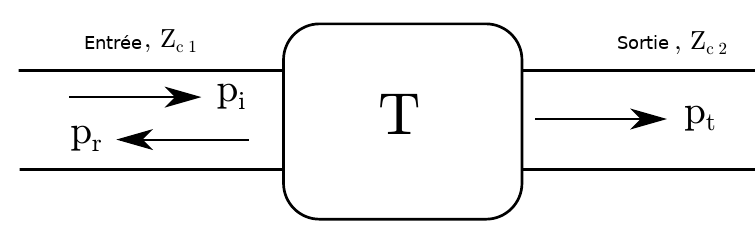
\includegraphics[ width=350px]{./images/th/scheme.png}
		\caption{Schéma matrice de transfert $T$ globale exprimé par la pression $p_1=p_i+p_r$ et $pt = p_2$}
		\label{schematrans2}
	\end{figure}
	La pression et la vélocité sont écrit du coté incident par :
	\begin{align}
	\begin{split}
	p_1&=p_i+p_r\\
	v_1&=\frac{(p_i-p_r)}{ Z_{c1}} \text{,}
	\label{eq:p1v1}
	\end{split}
	\end{align}
	la pression et la vélocité sont écris du coté transmis par :
	\begin{align}
	\begin{split}
	p_2&=p_t\\
	v_2&= \frac{p_t}{Z_{c2}}\text{.}
	\label{eq:p2v2}
	\end{split}
	\end{align}
	L'équation \ref{eq:p1v1} permet d'écrire : 
	\begin{equation}
	p_i = \frac{p_1 +v_1Z_{c1}}{2}\text{,}
	\end{equation}
	et en injectant $p_1$ et $v_1$ de l'Éq \ref{eq:Tglob2}:
	\begin{equation}
	p_i = \frac{T_{11}p_2+T_{12}v_2+Z_{c1}(T_{21}p_2+T_{22}v_2)}{2}\text{,}
	\end{equation}
	et en remplaçant les valeurs $p_2$ et $v_2$ par celles de l'Éq. \ref{eq:p2v2}:
	\begin{equation}
	p_i = \frac{T_{11}p_t+p_t\frac{T_{12}}{Z_{c2}}+p_tZ_{c1}(T_{21}+\frac{T_{22}}{Z_{c2}})}{2}\text{,}
	\end{equation}
	finalement on obtient en factorisant pat $p_t$ le ratio: 
	\begin{equation}
	\frac{p_i}{p_t} = \frac{1}{2} \left[T_{11}+\frac{T_{12}}{Z_{c2}}+Z_{c1}T_{21}+Z_{c1}\frac{T_{22}}{Z_{c2}}\right]\text{.}
	\label{eq:ratiopipt}
	\end{equation}
	On peut maintenant exprimer le coefficient de transparence Éq.\ref{eq:Tautrans} depuis le ratio trouvé Éq. \ref{eq:ratiopipt} : 
	\begin{equation}
	\tau =4  \frac{ \Re\left\lbrace Z_{c1} \right\rbrace}{\Re\left\lbrace Z_{c2}\right\rbrace} \left\|T_{11}+\frac{T_{12}}{Z_{c2}}+Z_{c1}T_{21}+Z_{c1}\frac{T_{22}}{Z_{c2}}\right\|^{-2}\text{.}
	\end{equation}
	L'indice d'affaiblissement peut donc s'écrire simplement par :
	\begin{equation}
	R = 10 \log_{10}\frac{ \Re\left\lbrace Z_{c1} \right\rbrace}{\Re\left\lbrace Z_{c2}\right\rbrace}+20 \log_{10}\left( \left\|T_{11}+\frac{T_{12}}{Z_{c2}}+Z_{c1}T_{21}+Z_{c1}\frac{T_{22}}{Z_{c2}}\right\|\right)-6
	\end{equation} 
	et dans le cas spécial d'air de chaque coté :
	\begin{equation}
	R = 20 \log_{10} \left\|T_{11}+\frac{T_{12}}{\rho_0 c_0}\cos\theta+\frac{\rho_0 c_0T_{21}}{\cos\theta}+T_{22}\right\|-6
	\end{equation}\\
	
	\chapter{Démonstration du système d'équation d'une plaque double avec un matériau poreux au milieu }
	\label{ch:demoporeux}
	\begin{align}
	\begin{cases}
	j k_0 \cos\theta (-1+A_{ref}) e^{-jk_0\sin\theta x_3} = -\rho_0\omega^2 C_{1}e^{-jkx_3}\\
	j k_p \cos\theta_p (-A_{tr2}+A_{ref2}) e^{-jk_p\sin\theta_p x_3} = -\rho_p\omega^2 C_{1}e^{-jkx_3}\\
	-\mu \omega^2C_{1}e^{-jkx_3}+Dk^4C_{1}e^{-jkx_3} = -e^{-jk_0\sin\theta x_3}-A_{ref}e^{-jk_0\sin\theta x_3}+A_{tr2}e^{-jk_p\sin\theta_p x_3}+A_{ref2}e^{-jk_p\sin\theta_p x_3}\\
	%
	j k_p \cos\theta (-A_{tr2}e^{-jk_p\cos\theta_p e}+A_{ref2}e^{+jk_p\cos\theta_p e})e^{-jk_p\sin\theta_p x_3}  = -\rho_p\omega^2 C_{2}e^{-jkx_3}\\
	j k_0\cos\theta (-A_{tr3}) e^{-jk_0\sin\theta x_3-jk_0\cos\theta e} = -\rho_0\omega^2 C_{2}e^{-jkx_3}\\
	-\mu \omega^2C_{2}e^{-jkx_3}+Dk^4C_{2}e^{-jkx_3} = -A_{tr2}e^{-jk_p\sin\theta_p x_3-jk_p\cos\theta_p e}-A_{ref2}e^{-jk_p\sin\theta_p x_3+jk_p\cos\theta_p e}+A_{tr3}e^{-jk_0\sin\theta x_3-jk_0\cos\theta e}\text{.}\\
	\end{cases}
	\end{align}
	Les conditions de continuités de vitesse entre les milieux et les plaques entrainent : 
	\begin{equation}
	k_0 \sin\theta = k_p \sin\theta_p =k\text{.}
	\end{equation}
	L'angle $\theta_p$ peut être calculé par :
	\begin{equation}
	\theta_p = \arcsin\frac{k_0 \sin\theta}{k_p} \text{.}
	\end{equation}
	Le système devient : 
	\begin{align}
	\begin{cases}
	j k_0 \cos\theta A_{ref}  +\rho_0\omega^2 C_{1}=j k_0 \cos\theta \\
	j k_p \cos\theta_p (-A_{tr2}+A_{ref2})  +\rho_p\omega^2 C_{1}=0\\
	-\mu \omega^2C_{1}+Dk^4C_{1} +A_{ref} -A_{tr2}-A_{ref2} = -1\\
	j k_p \cos\theta_p (-A_{tr2}e^{-jk_p\cos\theta_p e}+A_{ref2}e^{+jk_p\cos\theta_p e}) +\rho_p\omega^2 C_{2} =0\\
	j k_0 \cos\theta (-A_{tr3}) e^{-jk\cos\theta e} +\rho_0\omega^2 C_{2}=0\\
	-\mu \omega^2C_{2}+Dk^4C_{2} +A_{tr2}e^{-jk_p\cos\theta_p e}+A_{ref2}e^{jk_p\cos\theta_p e}-A_{tr3}e^{-jk\cos\theta e}=0 \text{.}\\
	\end{cases}
	\end{align}
	
	Sous forme de système on obtient (en remplaçant $\cos \theta$ par $\Theta$ et $\cos \theta_p$ par $\Theta_p$ )
	\begin{align}	
	\begin{bmatrix}
	j k_0 \Theta    &0 & 0 &0&\rho_0\omega^2&0  \\
	0       & -j k_p \Theta_p & j k_p \Theta_p & 0 &\rho_p\omega^2 & 0  \\
	1       & -1 & -1 & 0 &-\mu \omega^2+Dk^4 & 0  \\
	0    &-j k_p \Theta_p e^{-jk_p\Theta_p e}   & j k_p \Theta_p e^{jk_p\Theta_p e}   &0&0&\rho_p\omega^2  \\
	0       & 0 & 0 &- j k_0 \Theta e^{-jk_0\Theta e} &0 & \rho_0\omega^2   \\
	0     & + e^{-jk_p\Theta_p e} & +e^{jk_p\Theta_p e} & - 	e^{-jk_0\Theta e} &0 & -\mu \omega^2+Dk^4  \\
	\end{bmatrix}
	\begin{Bmatrix}
	A_{ref} \\
	A_{tr2} \\
	A_{ref2}\\
	A_{tr3}\\
	C_{1} \\
	C_{2} 
	\end{Bmatrix}
	=\begin{Bmatrix}
	j k_0 \Theta \\
	0 \\
	-1\\
	0\\
	0 \\
	0
	\end{Bmatrix}
	\end{align}
	
	\chapter{ Dispositif de test}
	\begin{figure}[h]
		\begin{minipage}[c]{.45\linewidth}
			\begin{center}
				\makebox[0pt]{\includegraphics[width=250px,height=350px]{images/obj/HP.JPG}}
				\caption{Haut Parleur.}
				\label{HautParleur}
			\end{center}
		\end{minipage}
		\hfill
		\begin{minipage}[c]{.45\linewidth}
			\begin{center}
				\makebox[0pt]{\includegraphics[width=350px,height=350px]{images/th/dispositifdetest.JPG}}	
				\caption{Dispositif de test}
				\label{Microsetautres}
			\end{center}
		\end{minipage}
	\end{figure}
	
	
\end{document}